\documentclass[a4paper,12pt]{article}
\usepackage{cmap}
\usepackage[T2A]{fontenc}
\usepackage[utf8]{inputenc}
\usepackage[english,russian]{babel}
\usepackage{listings}
\usepackage{amsmath}
\usepackage{amsfonts}
\usepackage{float}
\usepackage{csquotes}
\usepackage{graphicx}
\usepackage{hyphenat}
\usepackage{xcolor}
\usepackage{hyperref}
\usepackage{mathtools}
\usepackage{upgreek}


\renewcommand{\theequation}{\thesection.\arabic{equation}}


\author{Шерепа Никита}
\title{Лабораторная 12. GNU Radio.}
\date{\today}

\graphicspath{{res/screenshots}}

\begin{document}%
	
	\maketitle
	
	\newpage \tableofcontents
	\newpage \listoffigures
	
	\newpage
	
	\definecolor{dkgreen}{rgb}{0,0.6,0}
	\definecolor{gray}{rgb}{0.5,0.5,0.5}
	\definecolor{mauve}{rgb}{0.58,0,0.82}
	
	\lstset{
		language=Python,                 % выбор ЯП для подсветки 
		basicstyle=\small\sffamily, % размер и начертание шрифта для подсветки кода
		numbers=left,               % где поставить нумерацию строк (слева\справа)
		numberstyle=\tiny,           % размер шрифта для номеров строк
		stepnumber=1,                   % размер шага между двумя номерами строк
		numbersep=5pt,                % как далеко отстоят номера строк от подсвечиваемого кода
		aboveskip=3mm,
		belowskip=3mm,
		showstringspaces=false,
		columns=flexible,
		captionpos=b, 
		basicstyle={\small\ttfamily},
		numbers=left,
		numberstyle=\tiny\color{gray},
		keywordstyle=\color{blue},
		commentstyle=\color{mauve},
		stringstyle=\color{dkgreen},
		breaklines=true,
		breakatwhitespace=true,
		tabsize=3
	}

	\section{Передача сигнала}

	Первый этап - передача сигнала QPSK. Мы генерируем поток битов и модулируем его на сложное созвездие. Для этого мы используем блок \texttt{Constellation Modulator}, который использует \texttt{Constellation Rect} (созвездие)
	
	Объект созвездия позволяет нам определить, как кодируются символы. Затем блок модулятора использует эту схему модуляции с или без дифференциального кодирования. Также, для модулятора созвездия, используется генератор случайных битов со значениями от 0 до 255.
	
	Имея дело с количеством выборок на символ, мы хотим, чтобы это значение было как можно меньшим (минимальное значение 2). Здесь происходит моделирование количество отсчетов на символ важно только для того, чтобы обеспечить соответствие скорости передачи по всей потоковой диаграмме, здесь будет 4 что избыточно, но полезно для визуализации
	
	Также установим значение избыточной пропускной способности. Модулятор созвездия использует фильтр формирования импульсов RRC, который позволяет нам изменять один параметр для регулирования roll-off коэффициента фильтра - «альфа».
	
	Граф ниже визуализирует генерацию различных значений избыточной пропускной способности.
	
	\begin{figure}[H]
		\centering
		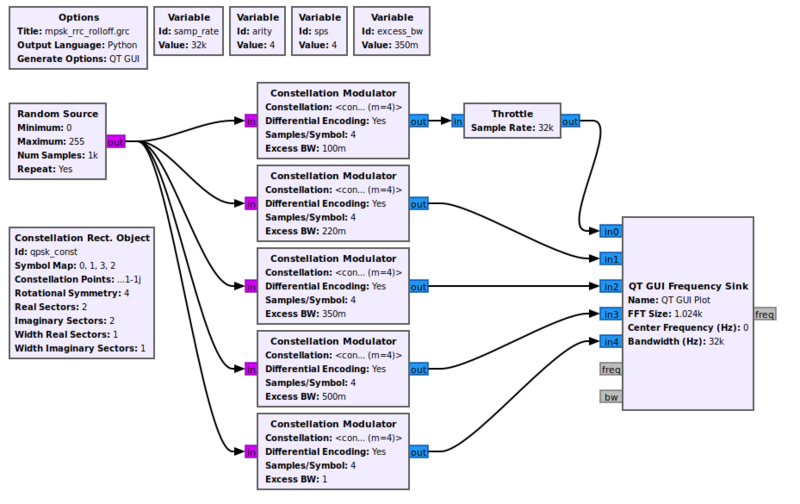
\includegraphics[width=0.75\textwidth]{1_1.png}
		\caption{mpsk\_rrc\_rolloff граф}
		\label{fig:1.1}
	\end{figure}

	Получаем следующий результат
	
	\begin{figure}[H]
		\centering
		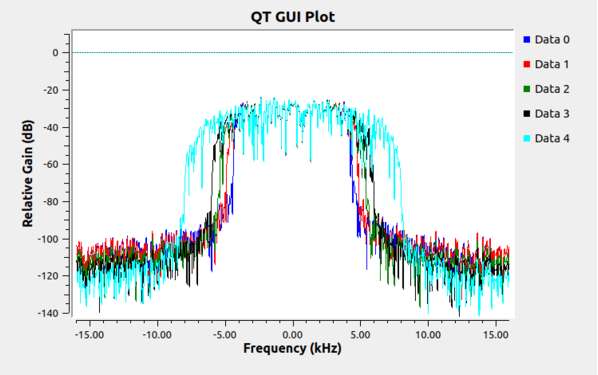
\includegraphics[width=0.75\textwidth]{1_2.png}
		\caption{Результат}
		\label{fig:1.2}
	\end{figure}
	
	Теперь рассмотрим граф, который передает созвездие \texttt{QPSK}. Он отображает передаваемый сигнал и часть цепи приемника во времени, частоте и диаграмме созвездия.
	
	\begin{figure}[H]
		\centering
		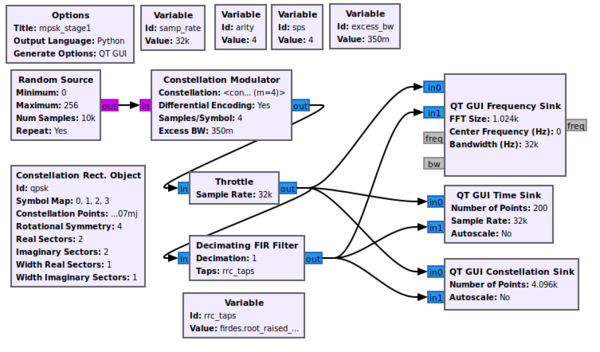
\includegraphics[width=0.75\textwidth]{1_3.png}
		\caption{mpsk\_stage1 граф}
		\label{fig:1.3}
	\end{figure}
	
	\begin{figure}[H]
		\centering
		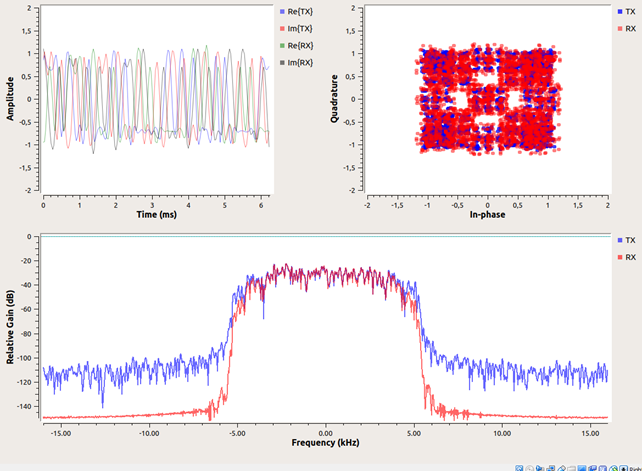
\includegraphics[width=0.75\textwidth]{1_4.png}
		\caption{Результат}
		\label{fig:1.4}
	\end{figure}
	
	Можно увидеть процесс фильтрации и эффект увеличения частоты дискретизации - генерирование 4х выборок на символ.
	
	На стороне приема мы избавляемся от ISI с помощью RRC фильтра. Фильтрация здесь просто свертка, поэтому выходной сигнал RRC-фильтра на приемной стороне представляет собой сигнал в форме приподнятого косинусоидального импульса с минимизированным ISI. 
	
	\newpage
	
	\section{Добавление канальных искажений}
	
	Теперь к передаче сигнала добавим искажений в канал передачи. Воспользуемся блоком \texttt{Channel Model}, который позволит смоделировать появление шума, а также различие тактовых сигналов, которые определяют частоту радиомодулей.
	
	Граф ниже позволяет экспериментировать с этими эффектами и наблюдать их влияние на сигнал.
	
	Выставим шум = 0.2, смещение частоты = 0.025, смещение времени = 1.0005
	
	\begin{figure}[H]
		\centering
		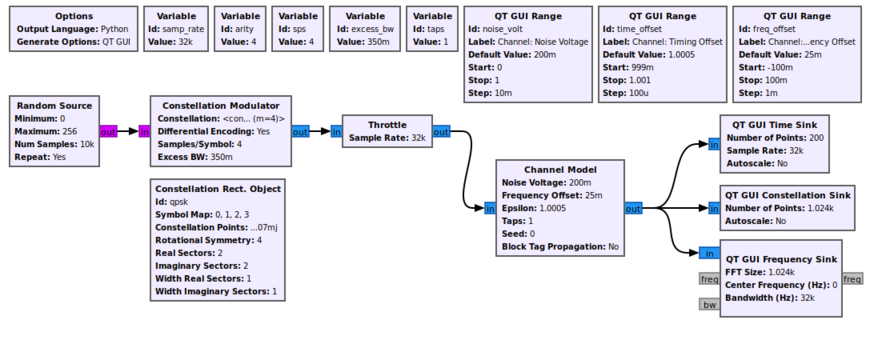
\includegraphics[width=0.75\textwidth]{2_1.png}
		\caption{mpsk\_stage2 граф}
		\label{fig:2.1}
	\end{figure}
	
	\begin{figure}[H]
		\centering
		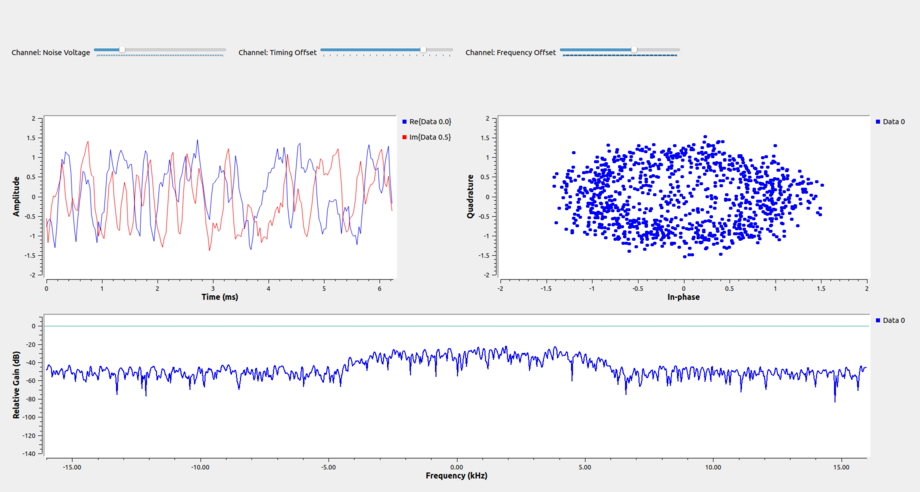
\includegraphics[width=0.75\textwidth]{2_2.png}
		\caption{Результат}
		\label{fig:2.2}
	\end{figure}
	
	Результат получился хуже, чем в прошлом пункте.
	
	\newpage
	
	\section{Временная коррекция}
	
	\subsection{Коррекция тактовых сигналов}
	
	Теперь попытаемся восстановить сигнал. Начнем с временного востановления. Попытаемся найти наилучшее время для дискретизации входящих сигналов, что позволит максимизировать \texttt{SNR} (отношение сигнал-шум) каждой выборки, а такэе уменьшить влияние \texttt{ISI} (межсимвольных помех). 
	
	Создадим четыре отдельных символа из единиц и отфильтруем их.
	
	\begin{figure}[H]
		\centering
		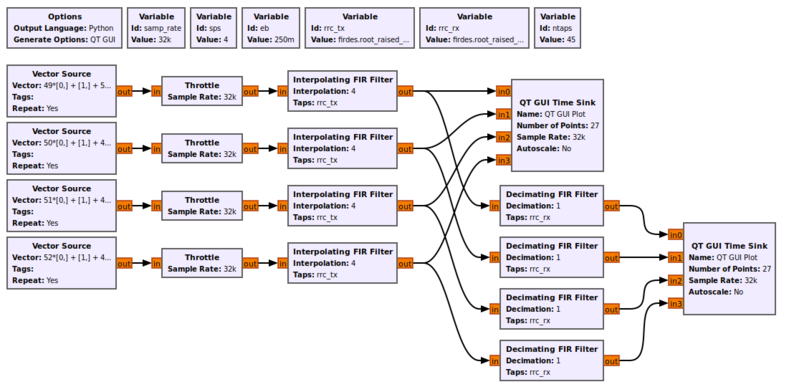
\includegraphics[width=0.75\textwidth]{3_1.png}
		\caption{symbol\_sampling граф}
		\label{fig:3.1}
	\end{figure}

	\begin{figure}[H]
		\centering
		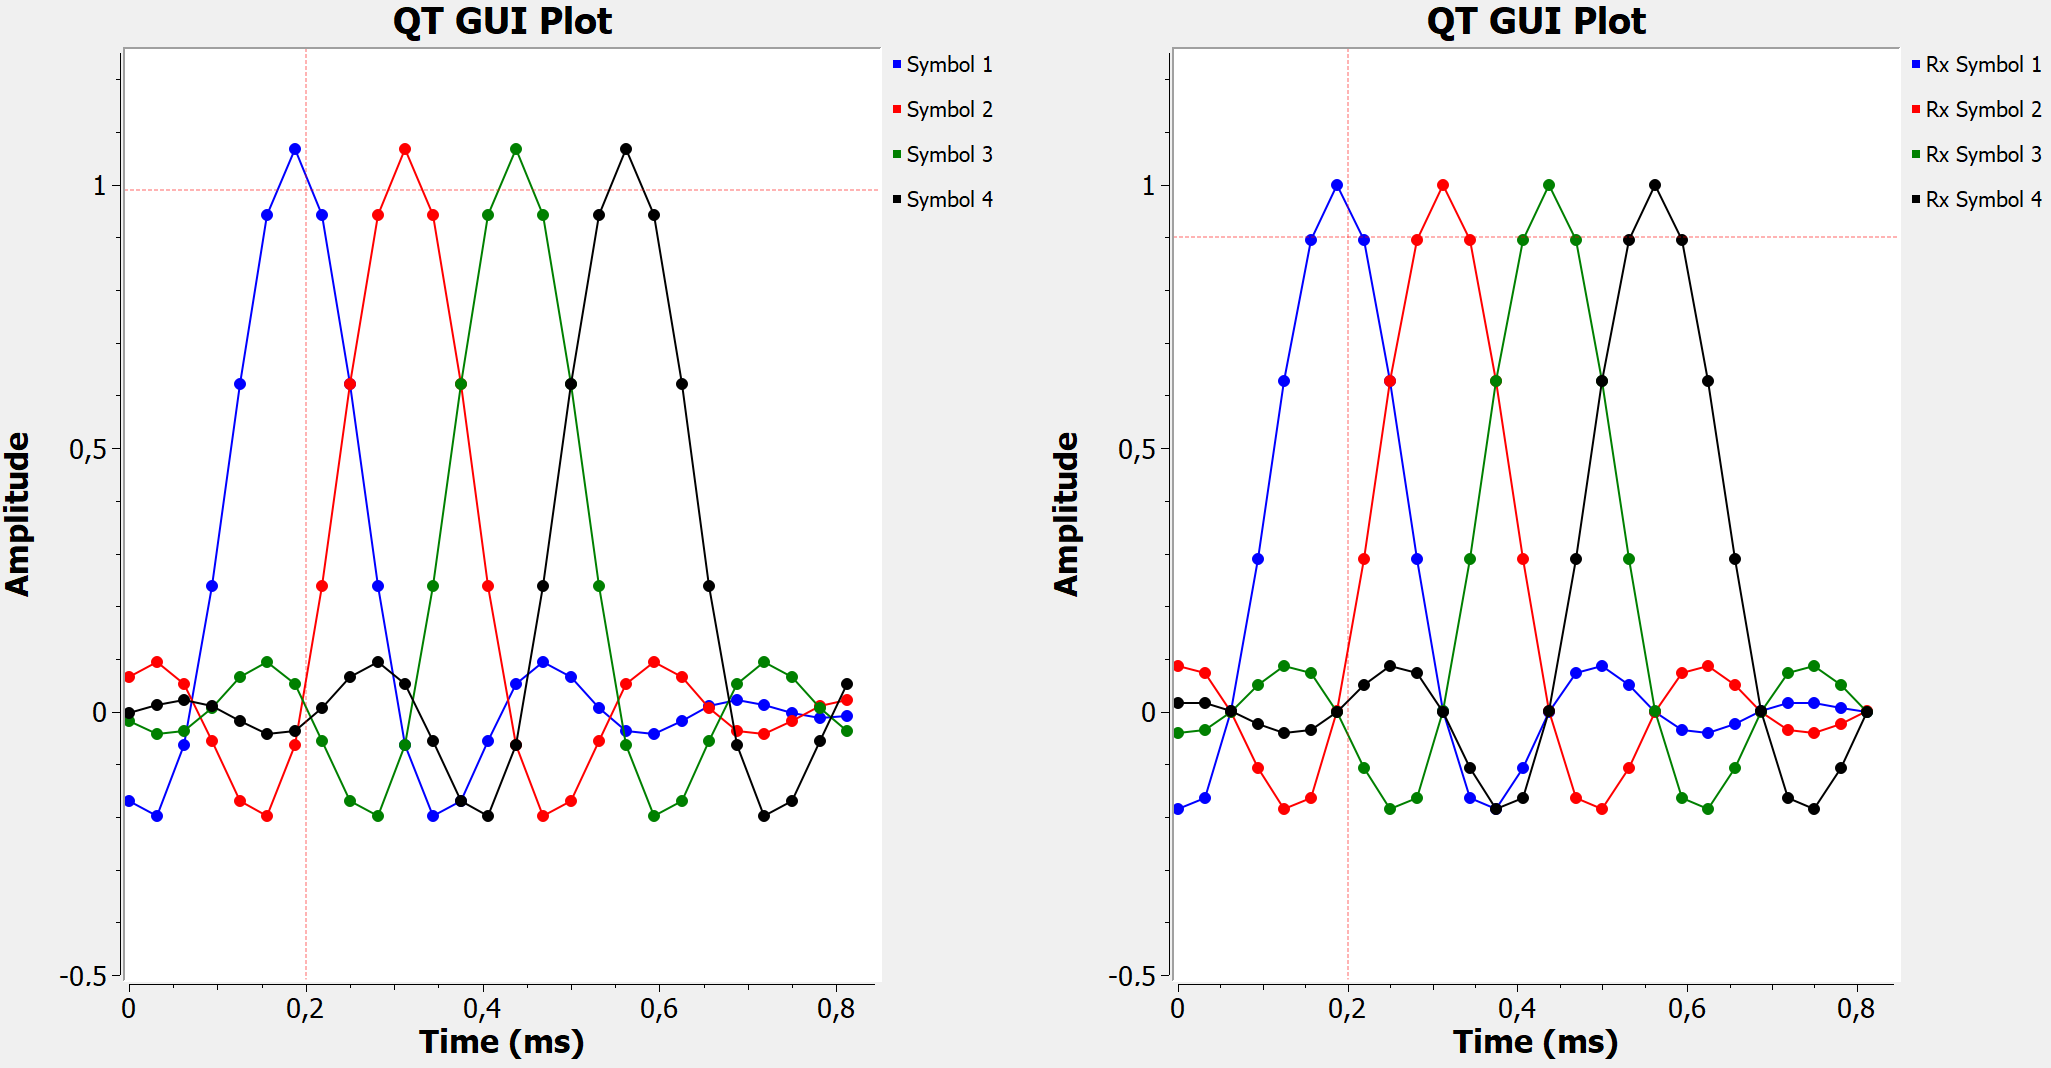
\includegraphics[width=0.75\textwidth]{3_2.png}
		\caption{Результат}
		\label{fig:3.2}
	\end{figure}
	
	Теперь рассмотрим влияние разных тактовых сигналов на точки выборки между передатчиком и приемником. Для модуляции этого добавим \texttt{Resampler}, который регулирует время выборки сигнала между переданным сигналом и приёмником.
	
	\begin{figure}[H]
		\centering
		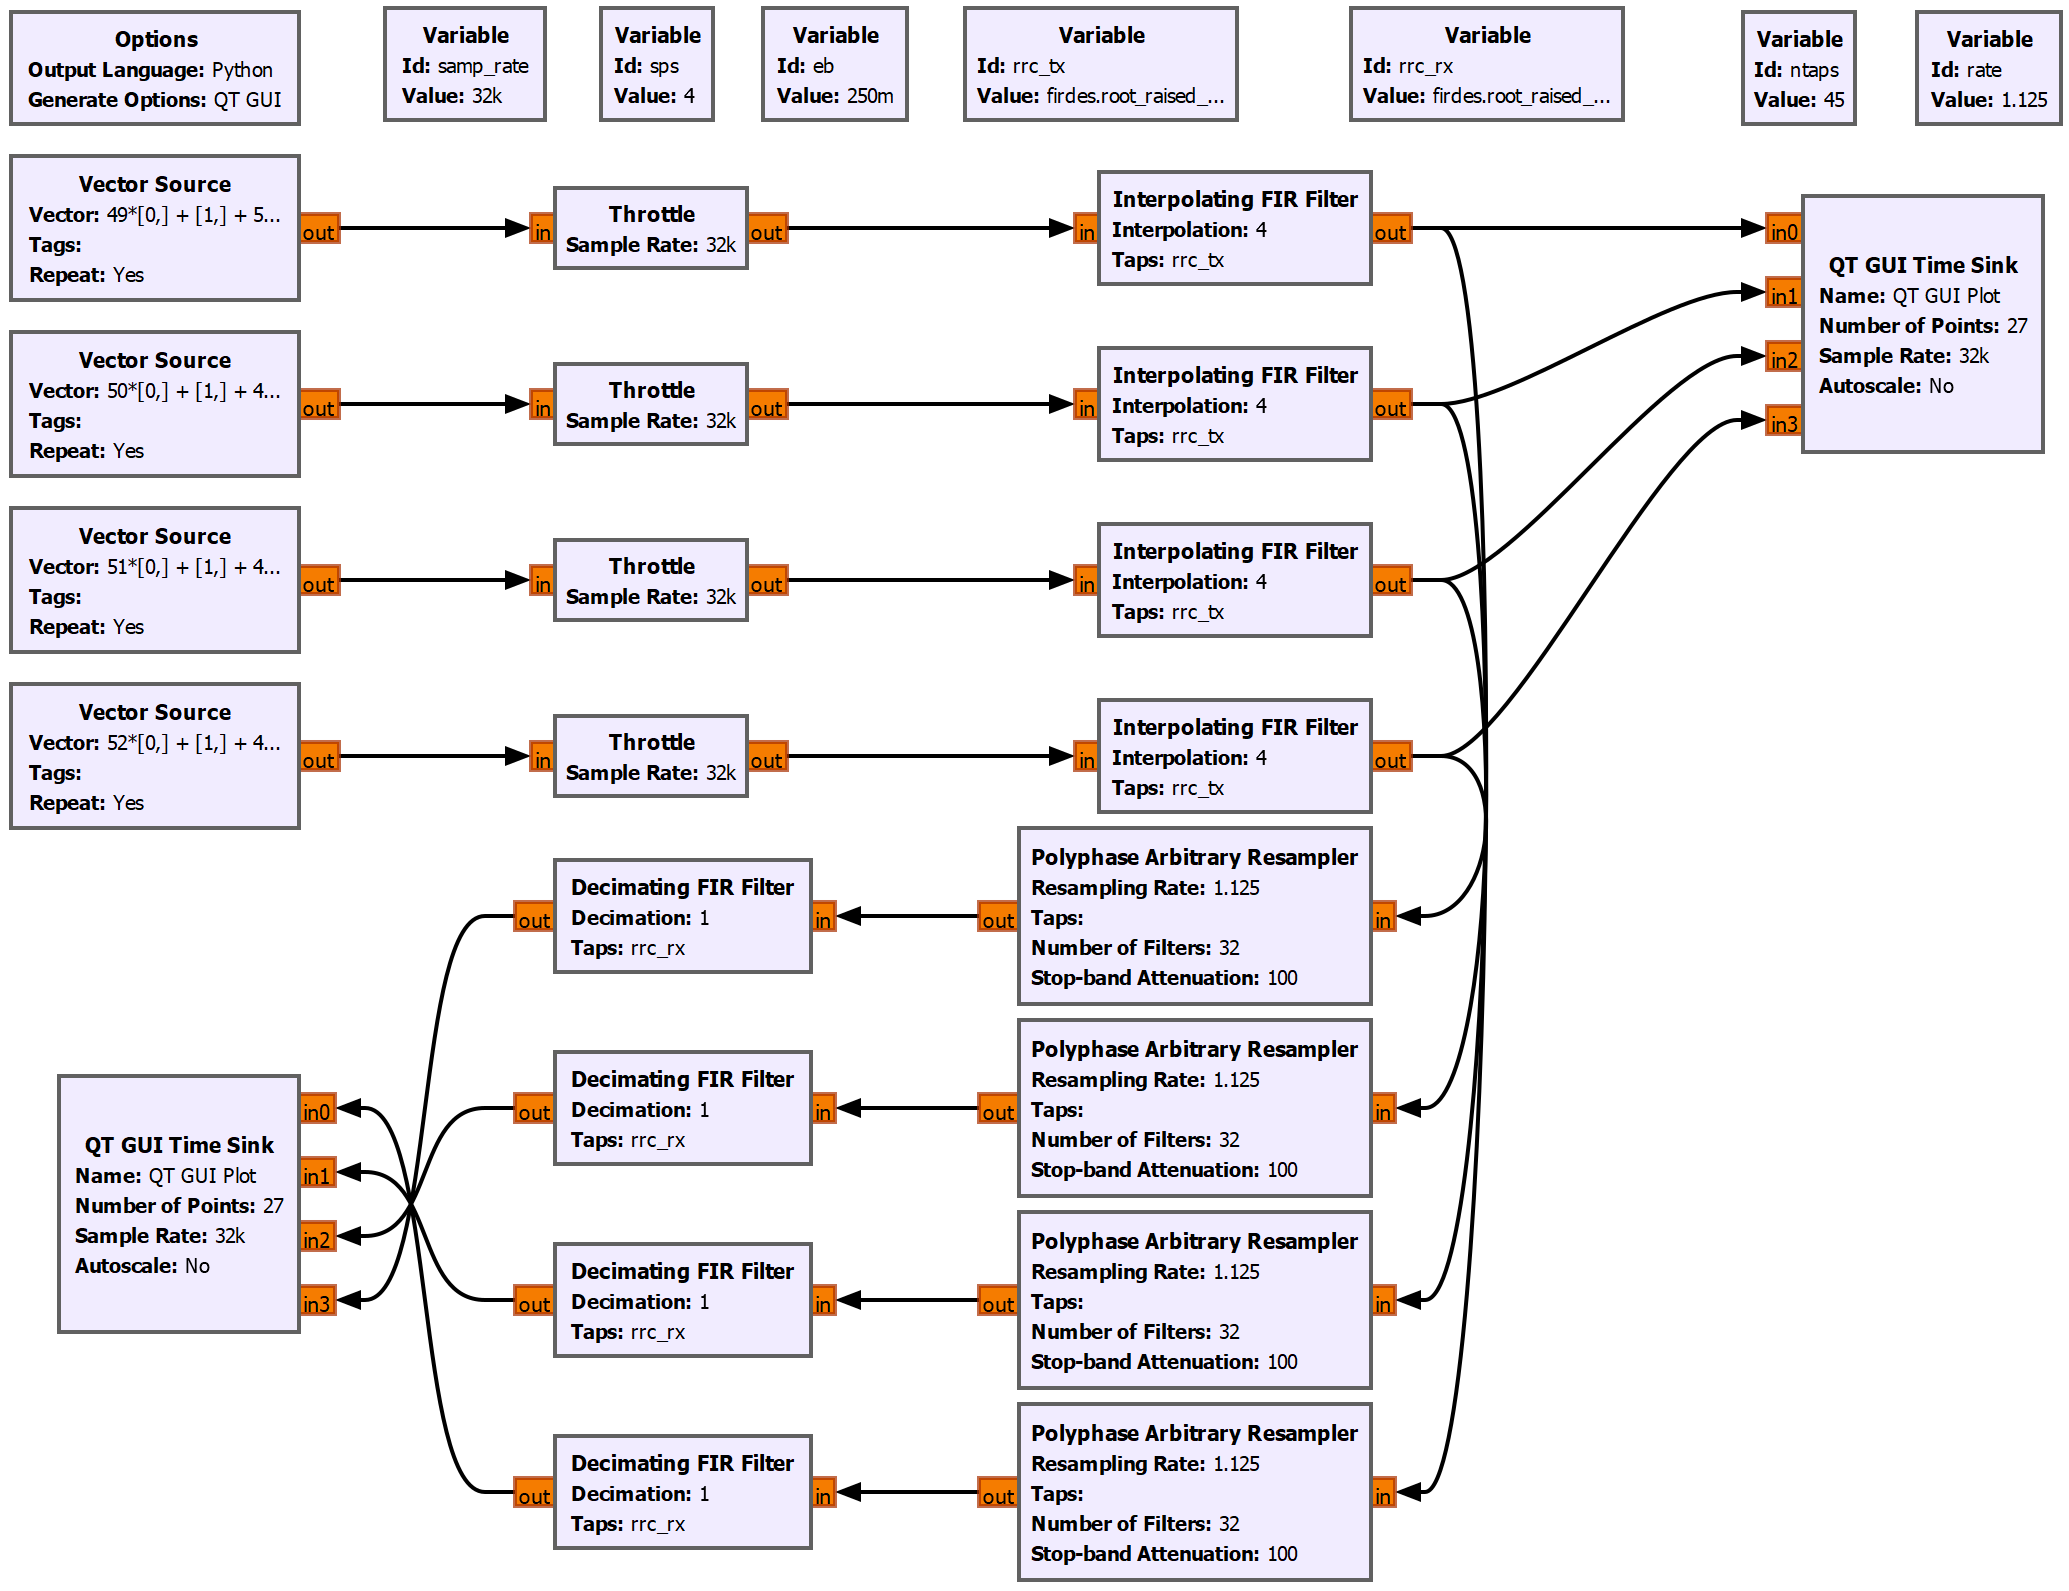
\includegraphics[width=0.75\textwidth]{3_3.png}
		\caption{symbol\_sampling\_diff граф}
		\label{fig:3.3}
	\end{figure}

	\begin{figure}[H]
		\centering
		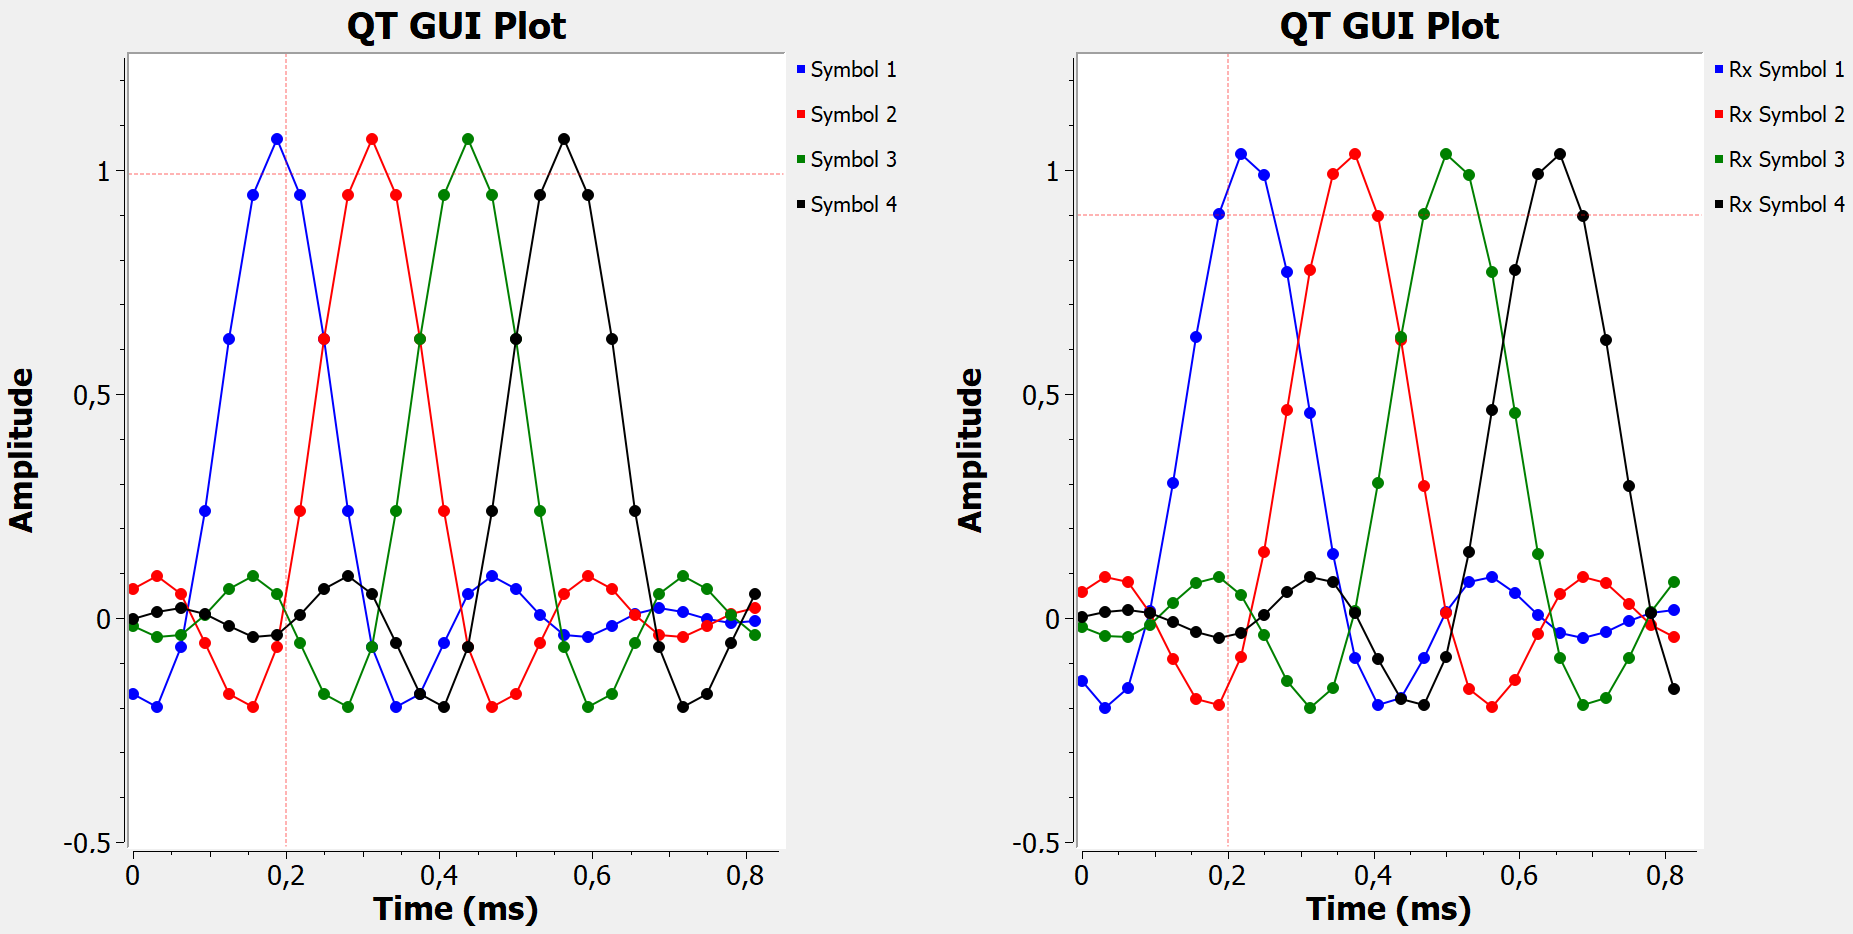
\includegraphics[width=0.75\textwidth]{3_4.png}
		\caption{Результат}
		\label{fig:3.4}
	\end{figure}
	
	
	\subsection{Информация о блоке синхронизации тактовых сигналов}
	
	Функции, выполняемые блоком синхронизации
	
	\begin{enumerate}
		
		\item
		
		Восстановление тактовых сигналов
		
		\item
		
		Согласованная фильтрация приёмника для устранения \texttt{ISI}
		
		\item
		
		Уменьшение частоты дискретизации сигнала
		 
		
	\end{enumerate}
	
	Блок синхронизации вычисляет первый дифференциал входящего сигнала, который будет связан с его смещением тактовой частоты. 
	
	\begin{figure}[H]
		\centering
		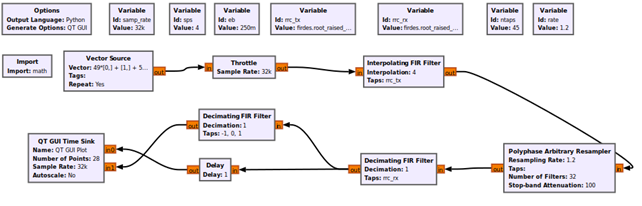
\includegraphics[width=0.75\textwidth]{3_5.png}
		\caption{symbol\_differential\_filter граф}
		\label{fig:3.5}
	\end{figure}
	
	\begin{figure}[H]
		\centering
		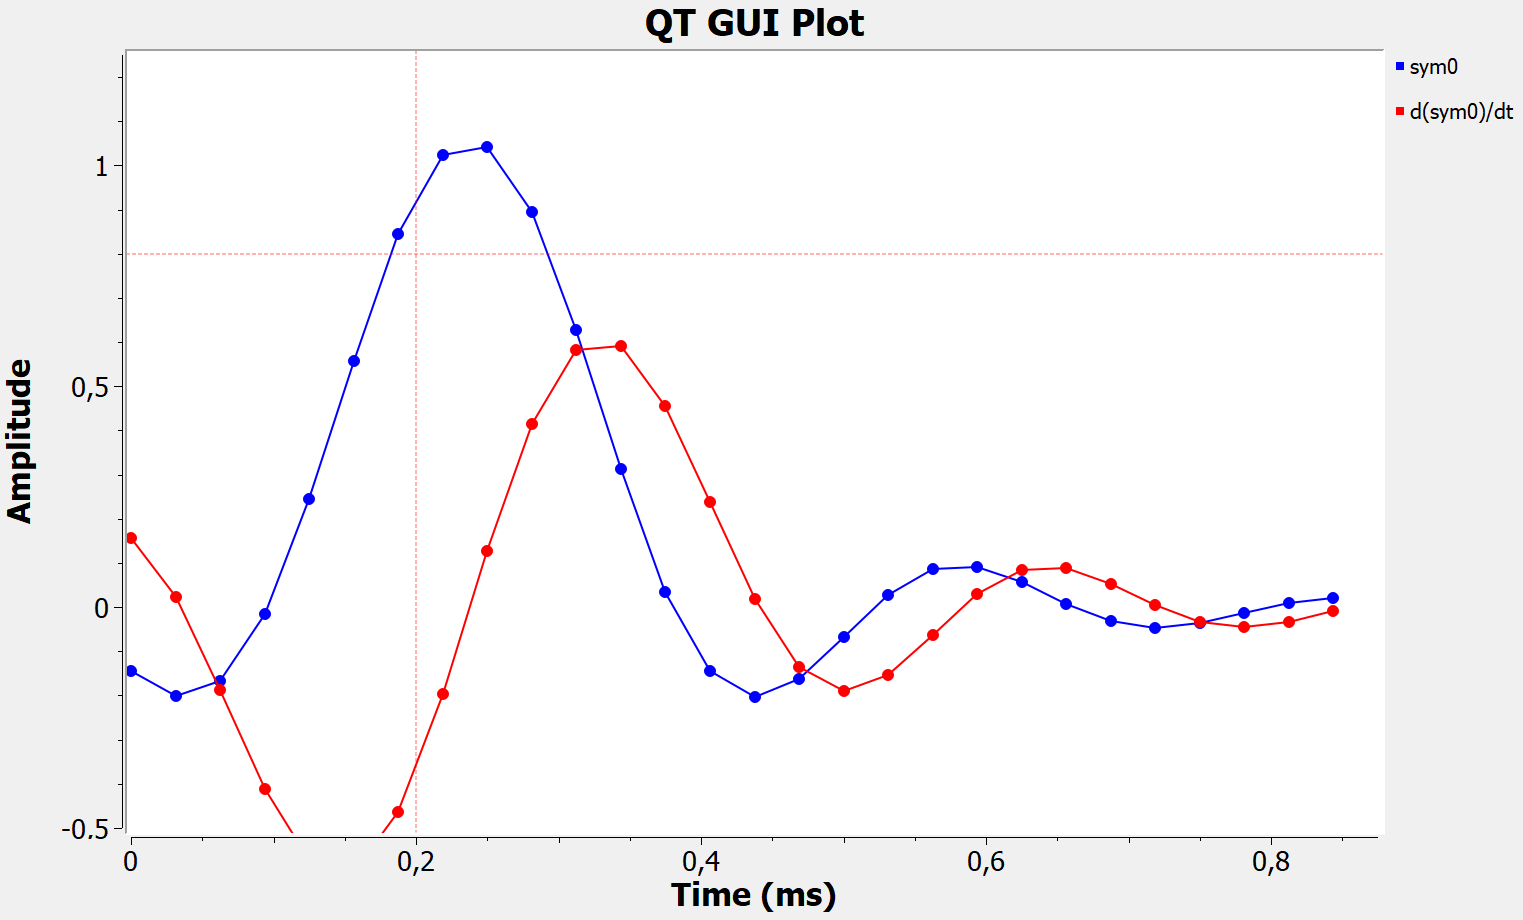
\includegraphics[width=0.75\textwidth]{3_6.png}
		\caption{Результат}
		\label{fig:3.6}
	\end{figure}
	
	Попробуем добавить тактовое смещение
	
	\begin{figure}[H]
		\centering
		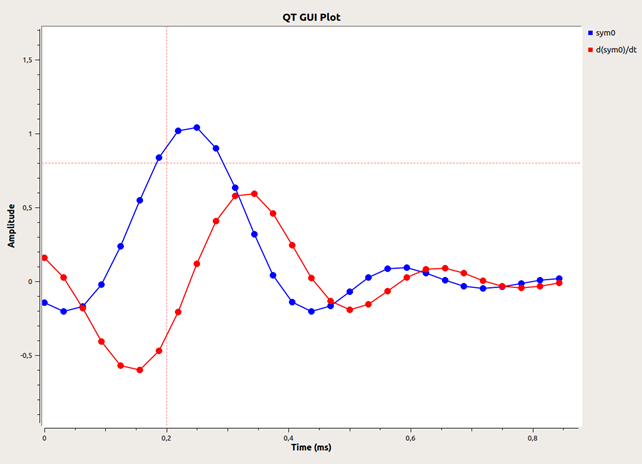
\includegraphics[width=0.75\textwidth]{3_7.png}
		\caption{Добавили тактовое смещение}
		\label{fig:3.6}
	\end{figure}

	Видим, что в пиковой точке дифференциальный фильтр уже не даёт 0.
	
	Вместо использования одного фильтра можно создать несколько фильтров с разной фазой. Из этих нескольких фильтров можно будет найти фильтр с правильной фазой, которая даст нужное значение синхронизации. 
	
	Проведем эксперимент с 5ю фильтрами.
	
	\begin{figure}[H]
		\centering
		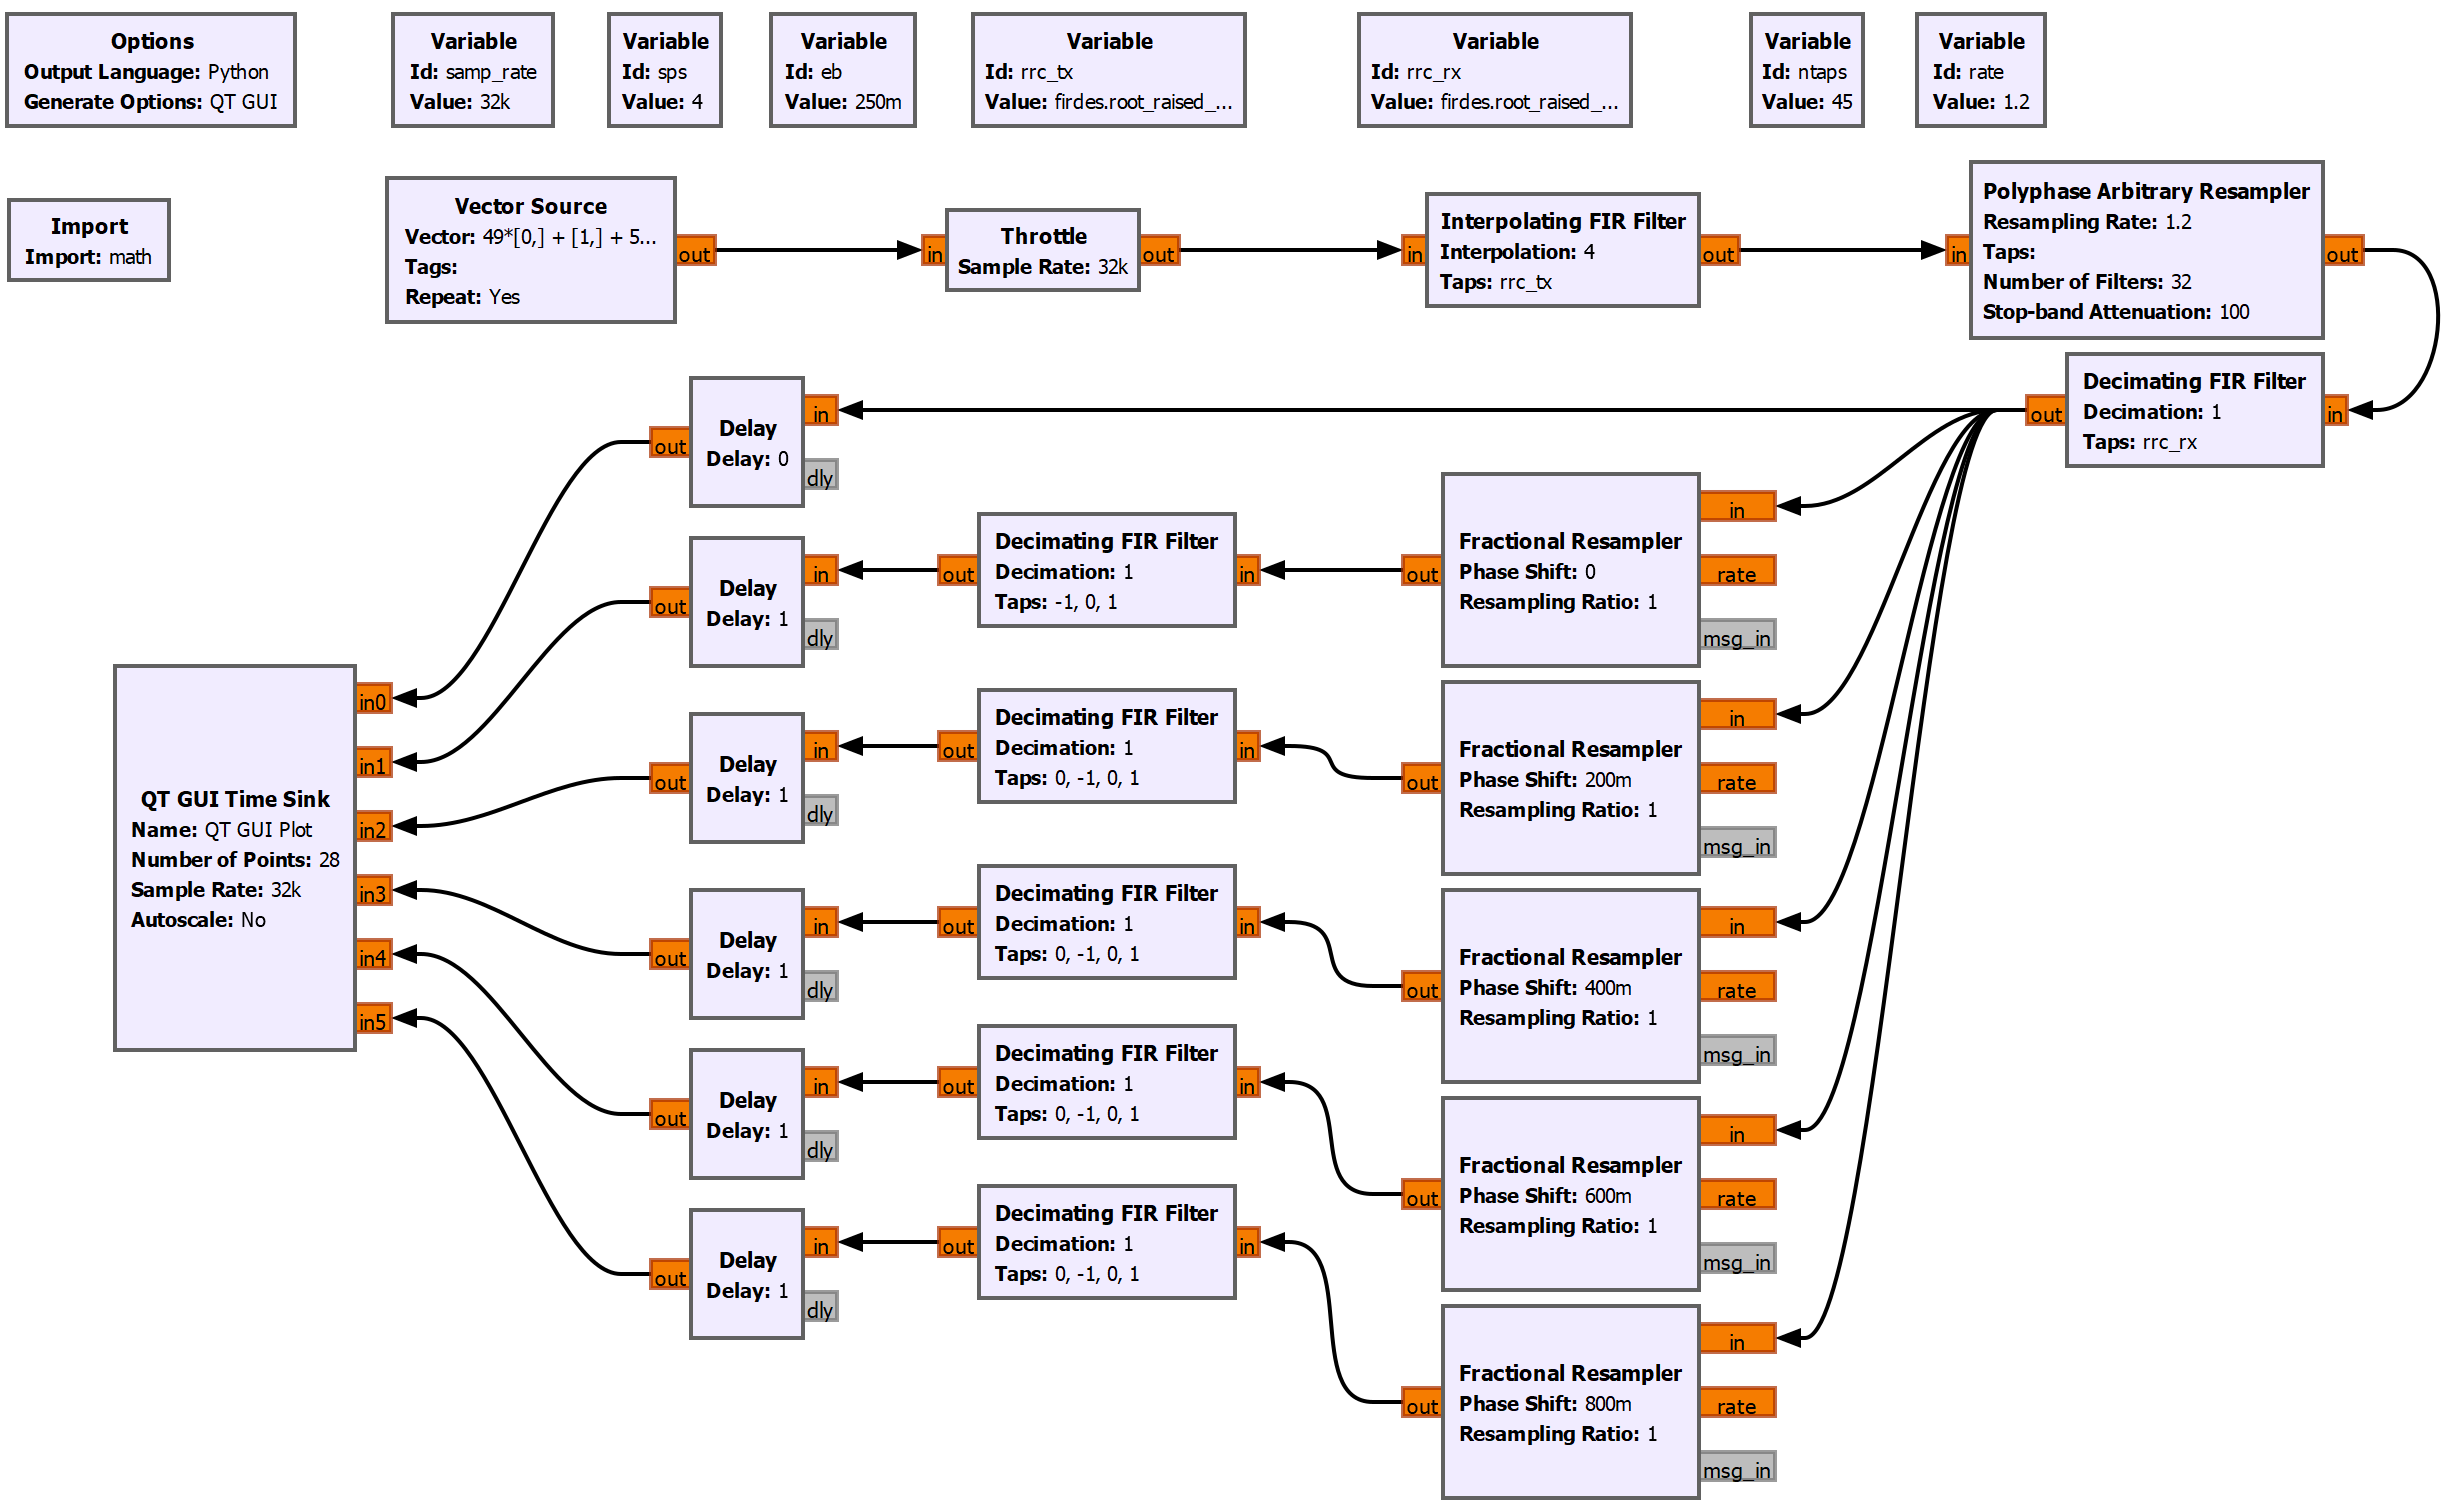
\includegraphics[width=0.75\textwidth]{3_8.png}
		\caption{5 фильтров}
		\label{fig:3.8}
	\end{figure}
	
	\begin{figure}[H]
		\centering
		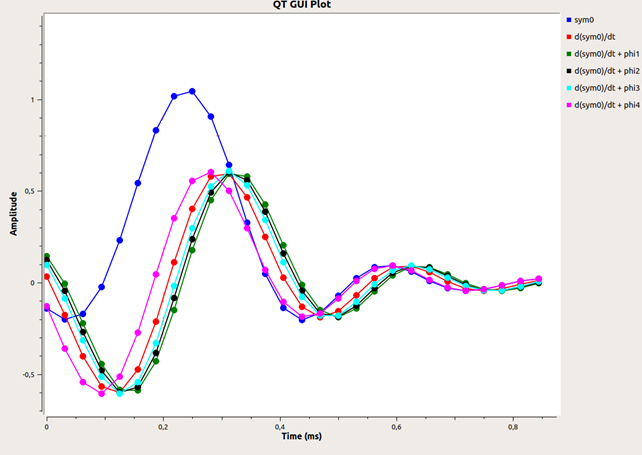
\includegraphics[width=0.75\textwidth]{3_9.png}
		\caption{Результат}
		\label{fig:3.9}
	\end{figure}

	Видим, что сигнал \texttt{d(sum0)/dt+ph3)} в правильной точке выборки даёт 0.
	
	\subsection{Использование блока многофазной синхронизации в приёмнике}
	
	Теперь используем этот блок синхронизации в приёмнике. Настроим его на использование 32 фильтров
	
	\begin{figure}[H]
		\centering
		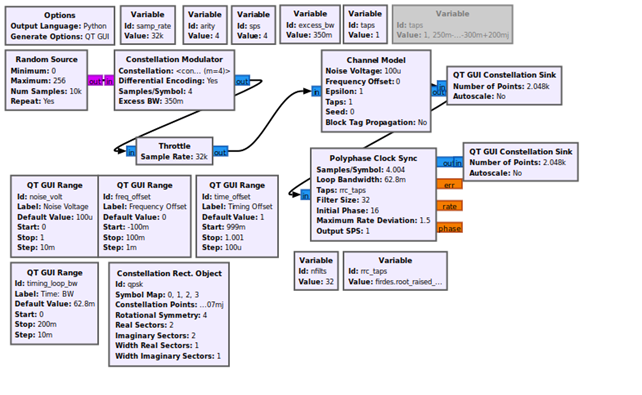
\includegraphics[width=0.75\textwidth]{3_10.png}
		\caption{mpsk\_stage3 граф}
		\label{fig:3.10}
	\end{figure}
	
	\begin{figure}[H]
		\centering
		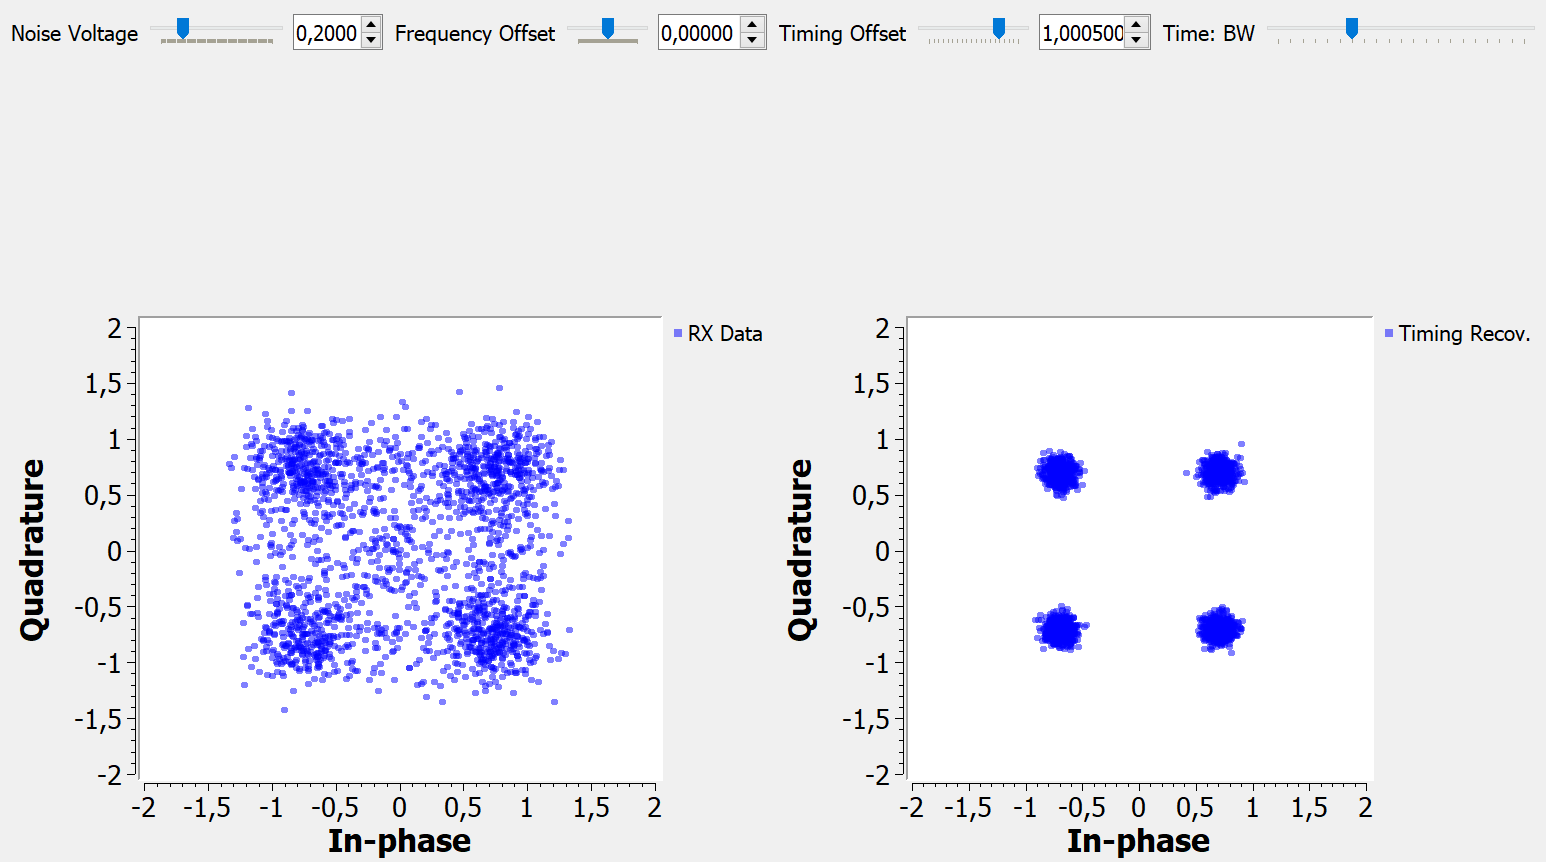
\includegraphics[width=0.75\textwidth]{3_11.png}
		\caption{Результат}
		\label{fig:3.11}
	\end{figure}
	
	Слева - сигнал до восстановления синхронизации
	
	Справа - сигнал после восстановления синхронизации
	
	\newpage
	
	\section{Многолучевое распространение}
	
	Бывает так, что на пути сигнала от передатчика к приемнику могут появится какие-нибудь объекты, отражающие сигнал - возникает искажение. В следствии этого, возникает многолучевое распространение - каждый раз сигнал будет проходить по разному пути и в разное время.
	
	Исправить это можно с помощью стерео-эквалайзера: можно усилить определенные частоты, чтобы подавить/усилить сигнал.
	
	\begin{figure}[H]
		\centering
		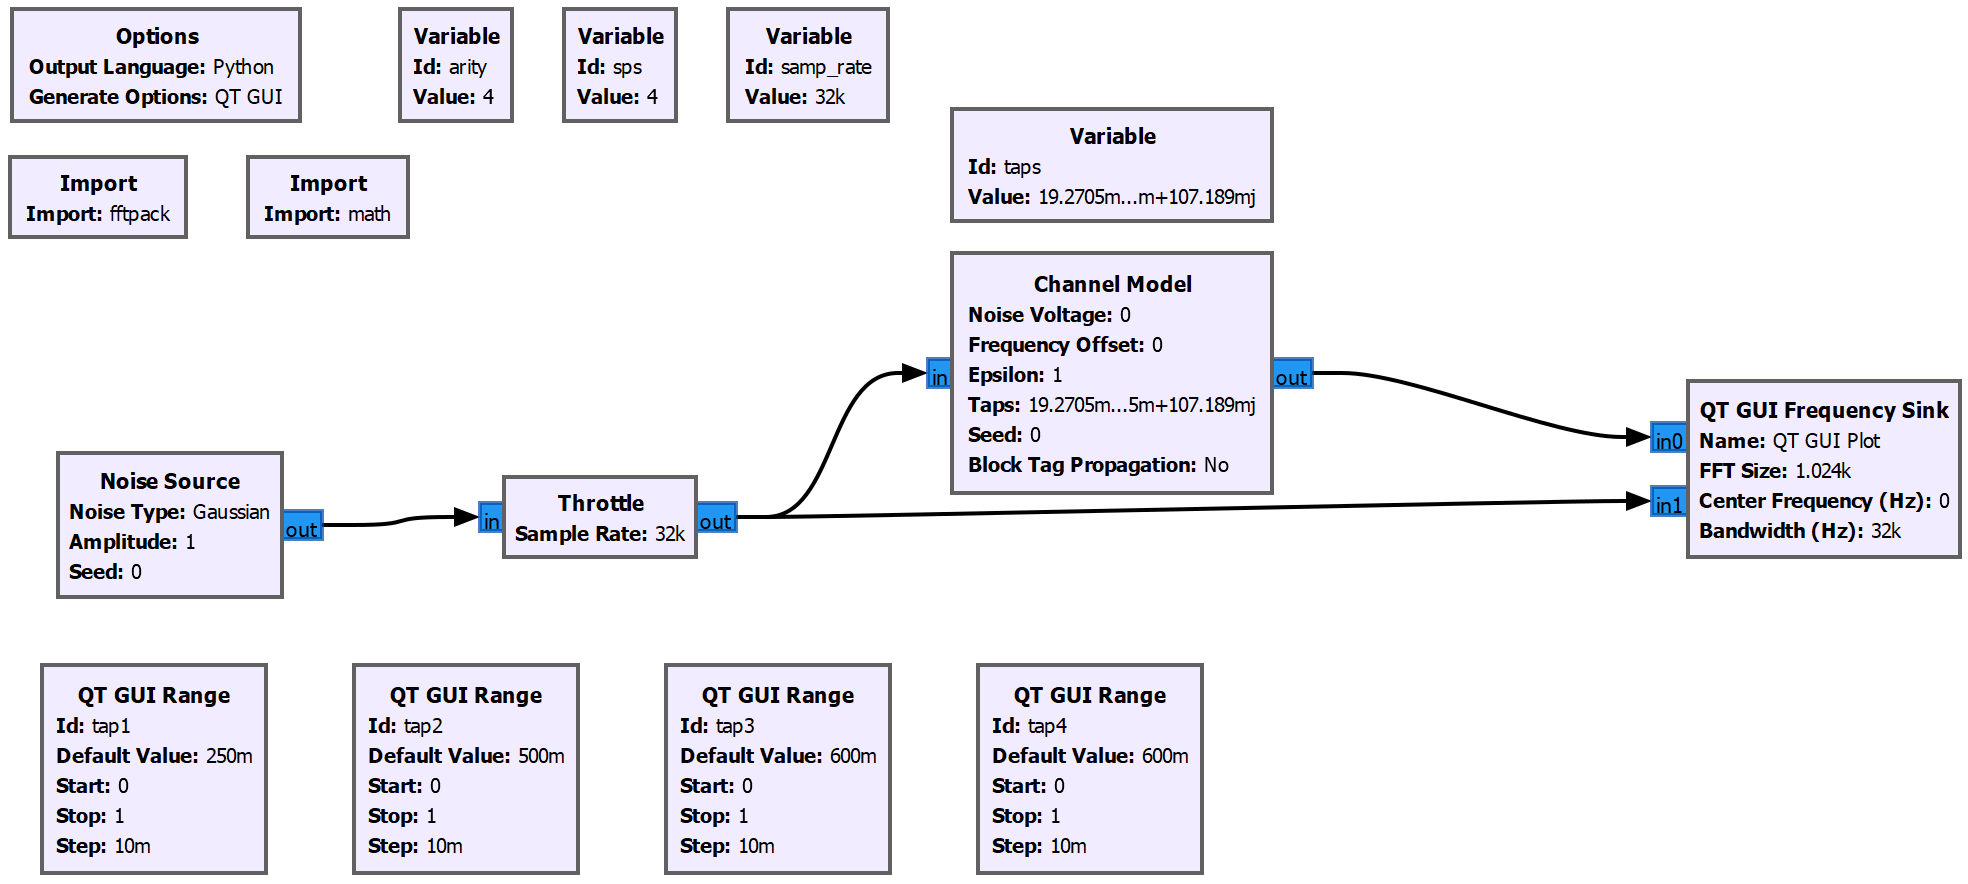
\includegraphics[width=0.75\textwidth]{4_1.png}
		\caption{multipath\_sim граф}
		\label{fig:4.1}
	\end{figure}
	
	Это моделирование настраивает модель канала, чтобы предоставить каналу пять элементов управления эквалайзером, четыре из которых мы можем изменить. Эти элементы управления настроены одинаково по частоте, и их можно настроить от 0 до 1. При значении 1 элемент управления позволит этим частотам проходить без помех. При значении 0 они будут производить глубокий ноль в спектре, который повлияет на все частоты вокруг него. График частоты установлен на среднее значение.
	
	\begin{figure}[H]
		\centering
		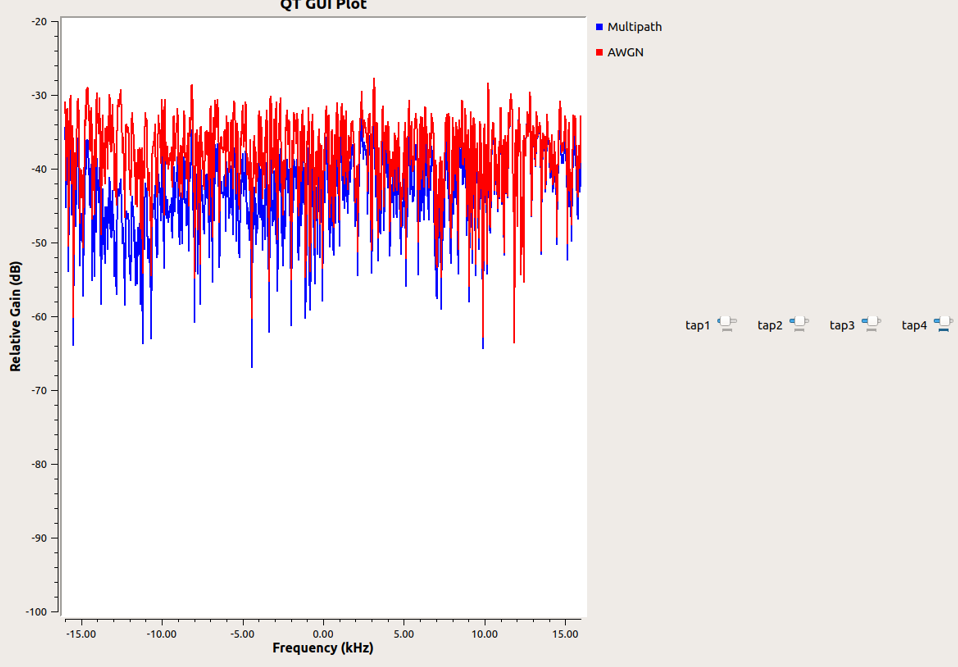
\includegraphics[width=0.75\textwidth]{4_2.png}
		\caption{Результат}
		\label{fig:4.2}
	\end{figure}
	
	Хотя в этом примере мы явно контролируем частотную область, на самом деле мы создаем эквалайзер, который может корректировать или регулировать частотную характеристику принятого сигнала. В итоге, многолучевой канал создает некоторые искажения в сигнале, как показано в частотной области. Задача эквалайзера - инвертировать этот канал.
	
	\newpage
	
	\section{Эквалайзеры}
	
	В GNU Radio используется два эквалайзера
	
	\begin{enumerate}
		
		\item
		
		\texttt{CMA Equalizer} - "слепой" эквалайзер, который работает только с сигналами с постоянной амплитудой или модулем
		
		\item
		
		\texttt{LMS-DD Equalizer} - должен знать точки созвездия, чтобы понимать, как обновлять параметры эквалайзера. Более сложен в вычислениях. Требует большей производительности.
		
	\end{enumerate}
	
	Рассмотрим работу \texttt{CMA Equalizer}. 
	
	\begin{figure}[H]
		\centering
		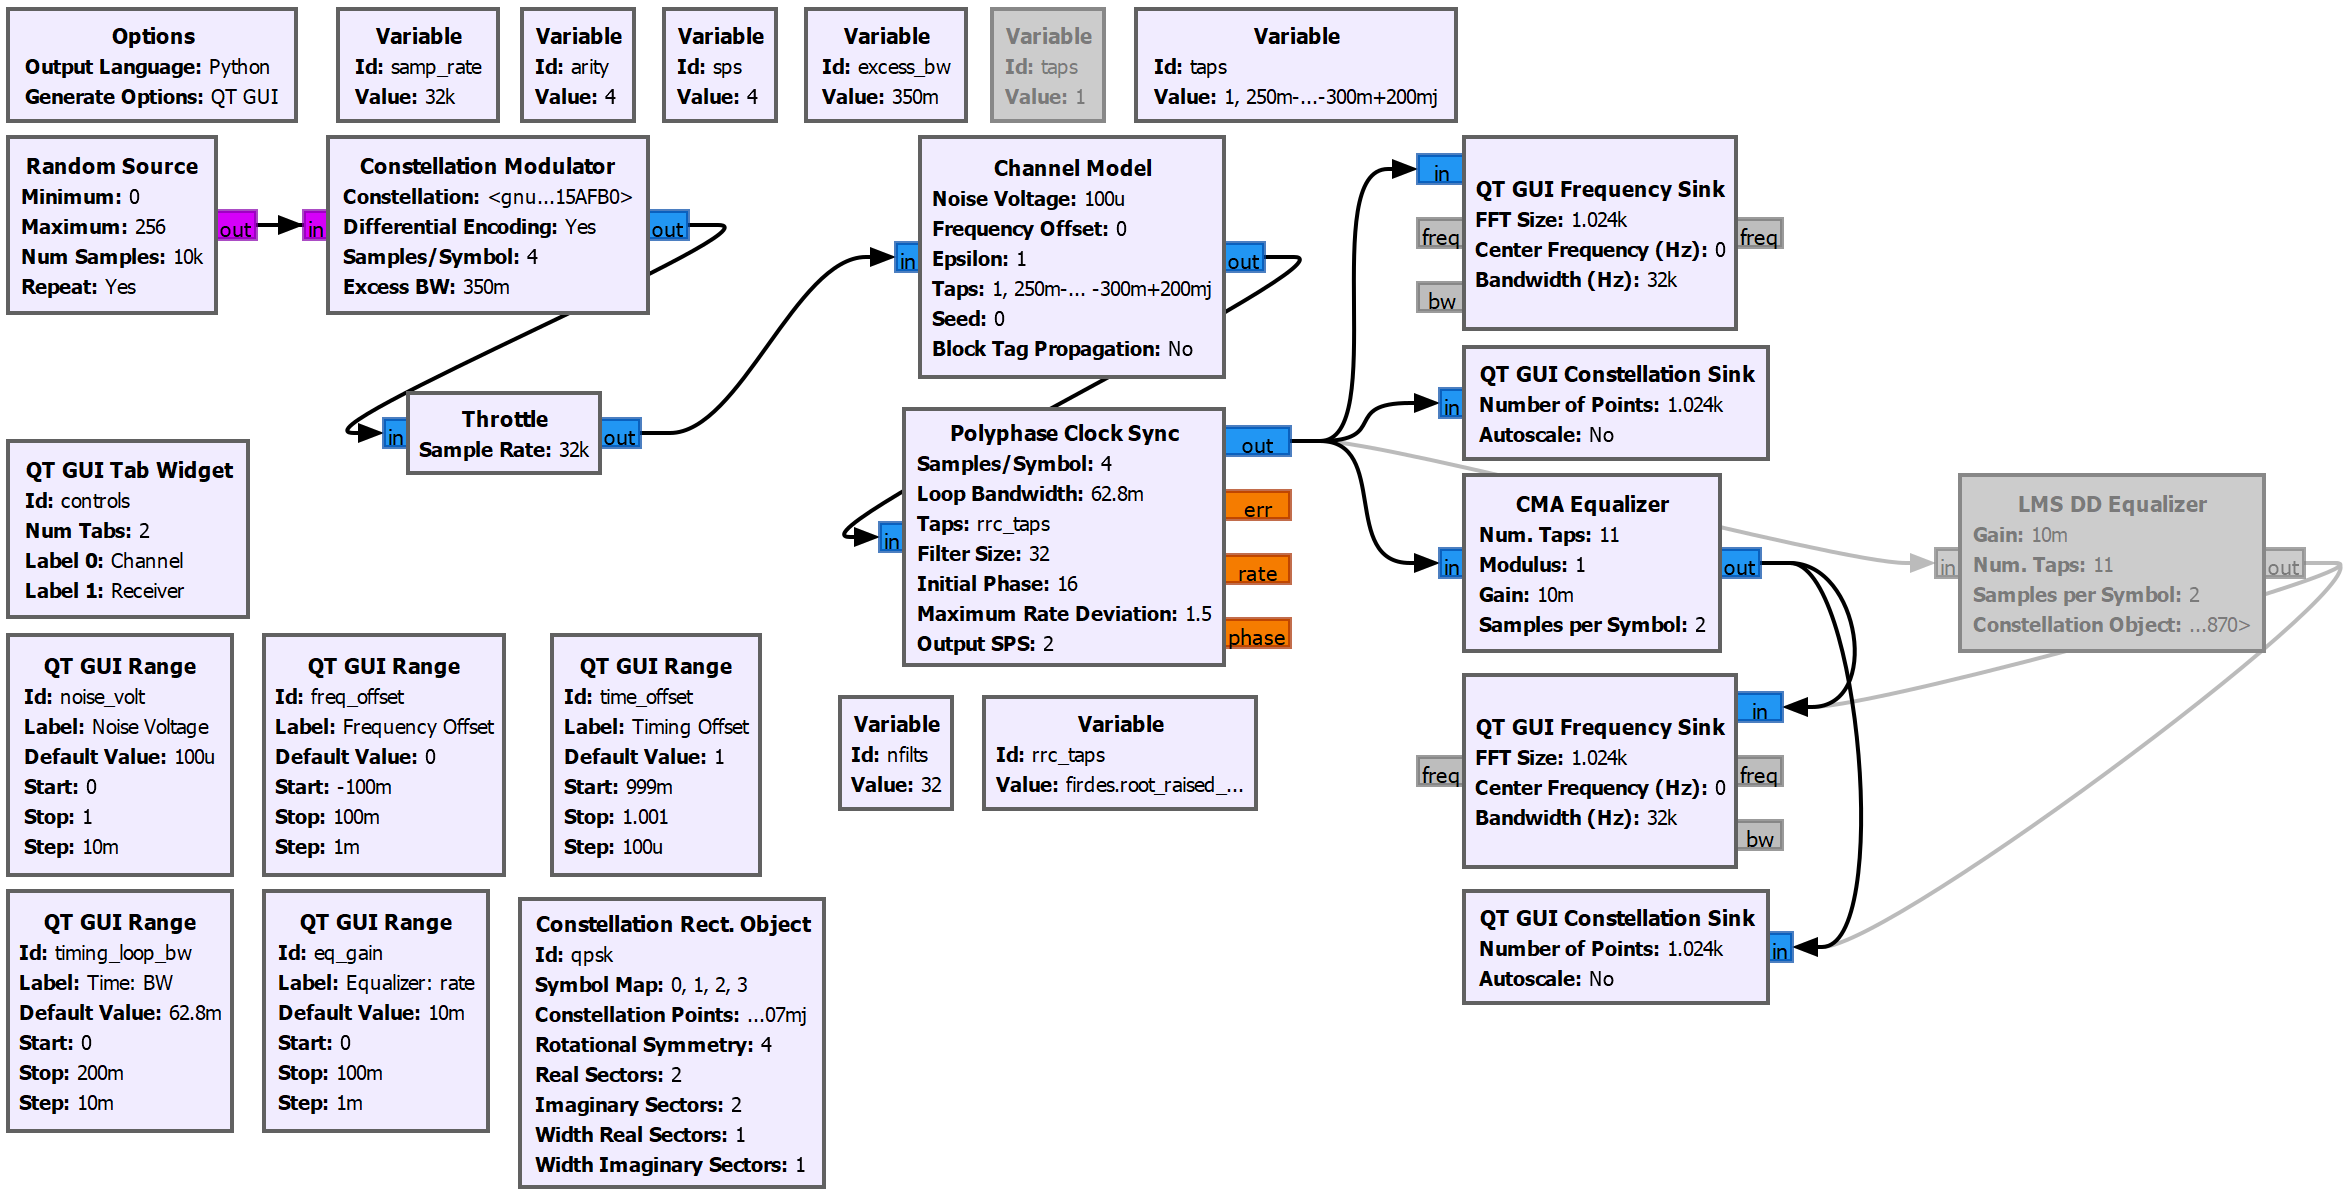
\includegraphics[width=0.75\textwidth]{5_1.png}
		\caption{mpsk\_stage4 граф с \texttt{CMA}}
		\label{fig:5.1}
	\end{figure}
	
	\begin{figure}[H]
		\centering
		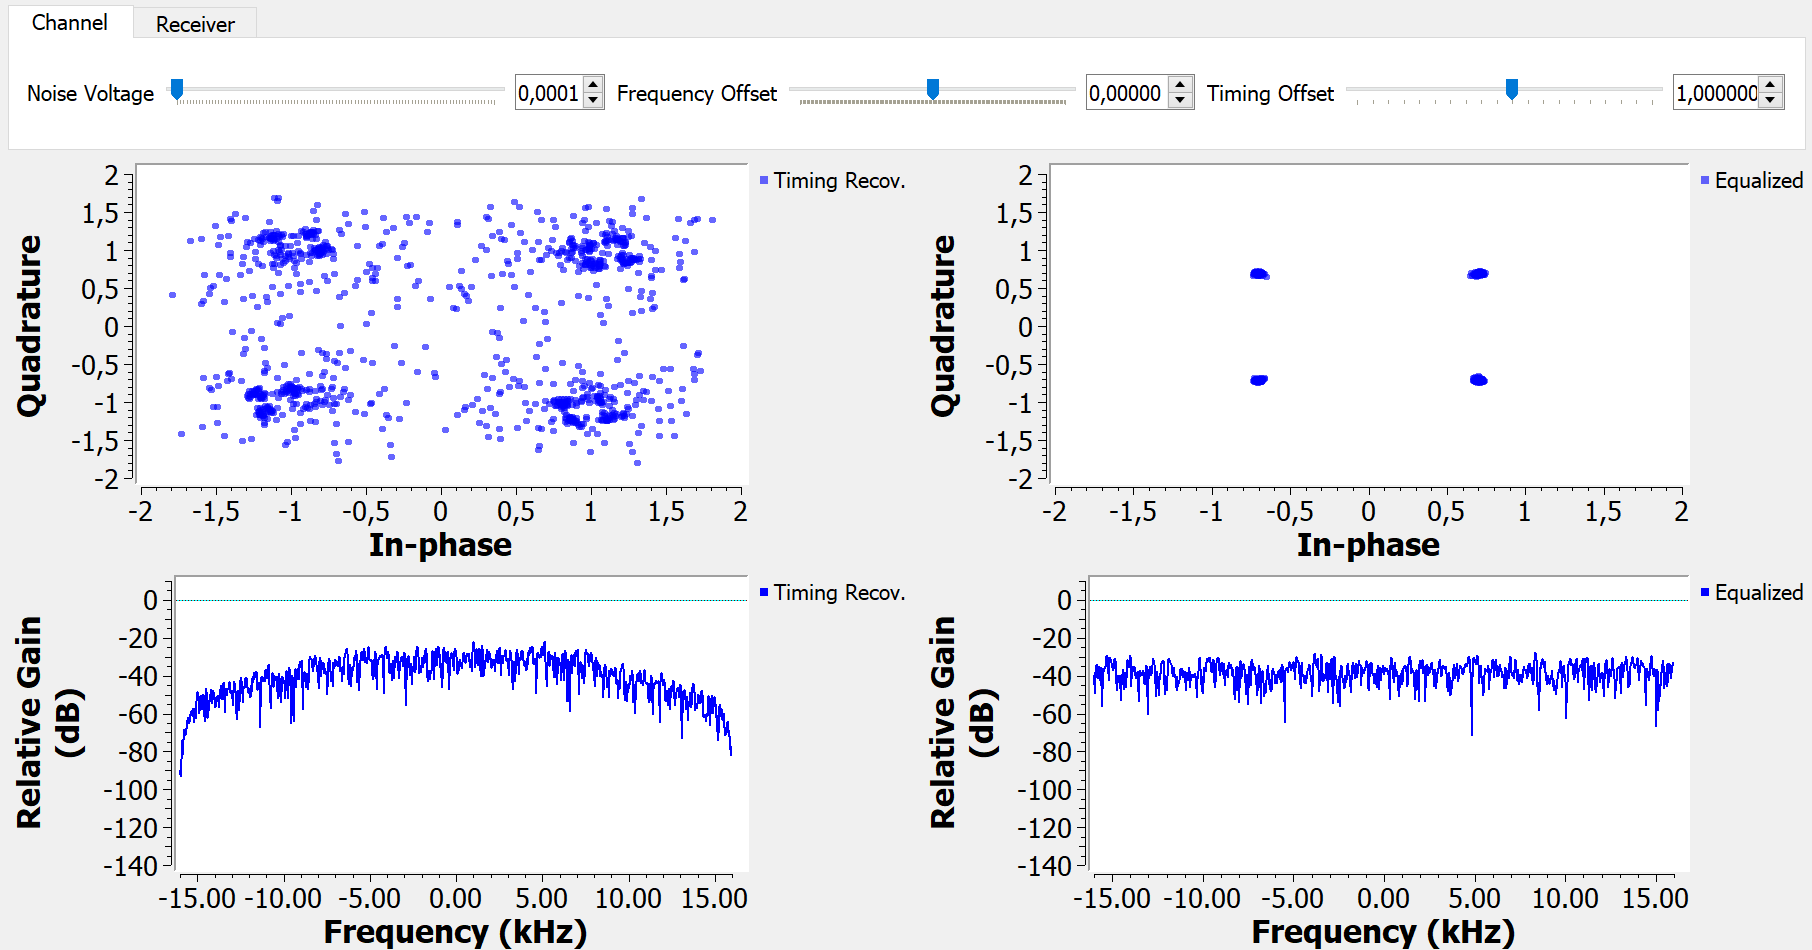
\includegraphics[width=0.75\textwidth]{5_2.png}
		\caption{Результат работы \texttt{CMA}}
		\label{fig:5.2}
	\end{figure}
	
	Видим эффект синхронизированного по времени многолучевого сигнала до и после эквалайзера. 
	
	Перед эквалайзером - некрасивый сигнал без шумов
	
	Эквалайзер понимает что нужно инвертировать, чтобы получился чистый сигнал.
	
	В конце концов видим, что канал выравнился после работы эквалайзера.
	
	Теперь рассмотрим работу \texttt{LMS-DD Equalizer}
	
	Этот эквалайзер хорошо подходит для сигналов, которые не подходят под требование постоянной амплитуды, поэтому его можно использовать и для QAM-модуляции.
	
	\begin{figure}[H]
		\centering
		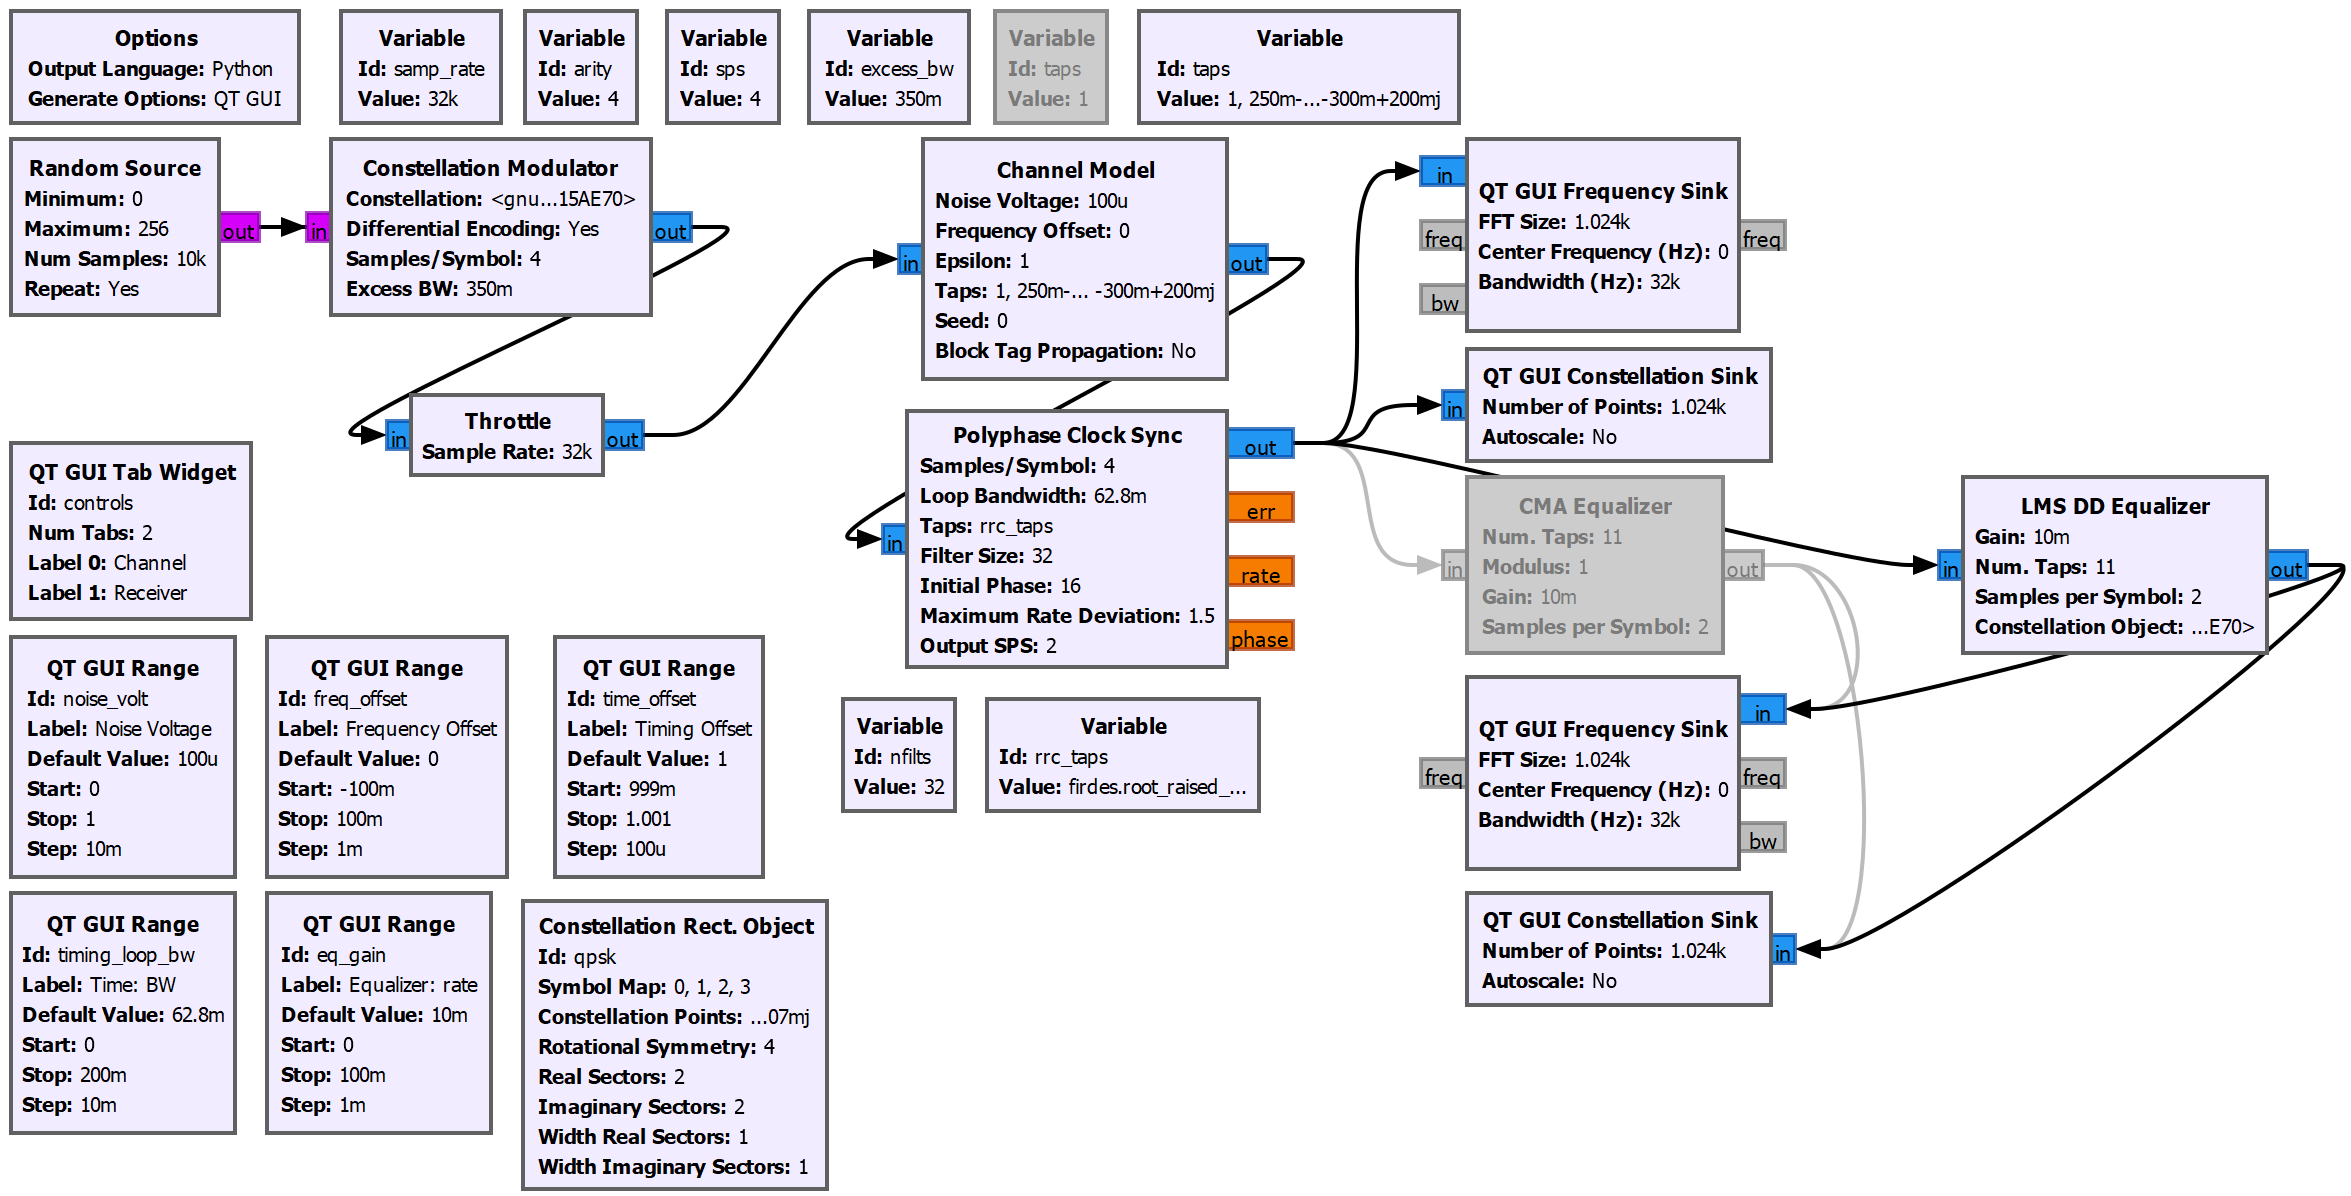
\includegraphics[width=0.75\textwidth]{5_3.png}
		\caption{mpsk\_stage4 граф с \texttt{LMS-DD}}
		\label{fig:5.3}
	\end{figure}
	
	\begin{figure}[H]
		\centering
		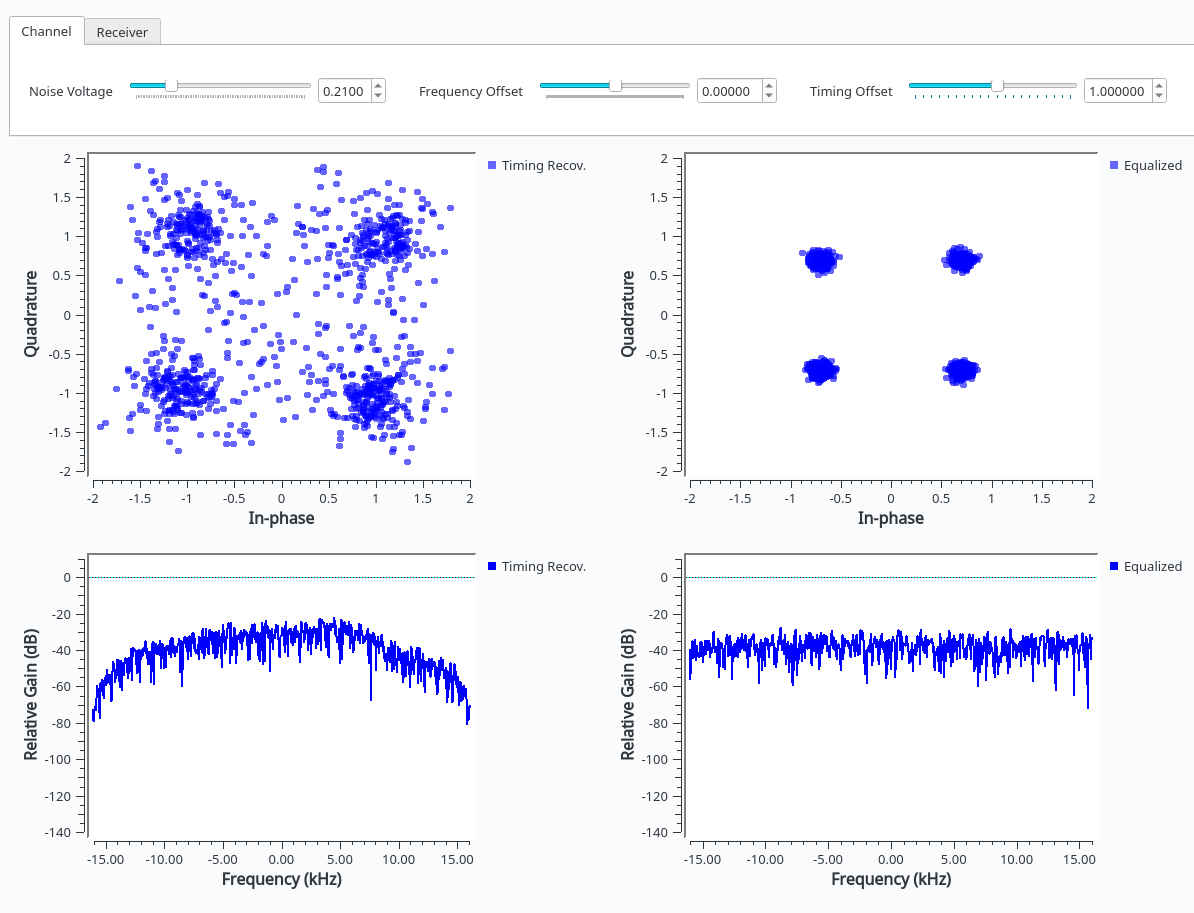
\includegraphics[width=0.75\textwidth]{5_4.png}
		\caption{Результат работы \texttt{LMS-DD}}
		\label{fig:5.4}
	\end{figure}
	
	Видим, что канал успешно выравнялся.
	
	
	\section{Фазовая и точная частотная коррекция}
	
	Учитывая, что мы выровняли канал, у нас все еще есть проблема смещения фазы и частоты. Эквалайзеры, как правило, не адаптируются быстро, поэтому смещение частоты может быть легко за пределами возможностей эквалайзера. Кроме того, если мы просто запускаем эквалайзер CMA, все, о чем он заботится, - это схождение к единичной окружности. Он ничего не знает о созвездии, поэтому, когда он блокируется, он блокируется на любой заданной фазе. Теперь нам нужно исправить любой сдвиг фазы, а также любой сдвиг частоты.
	
	Для этой задачи мы собираемся использовать цикл Костаса. Блок \texttt{Costas Loop} может синхронизировать \texttt{BPSK}, \texttt{QPSK} и \texttt{8PSK}. Приемник созвездия будет привязан к любому заданному объекту созвездия, хотя в зависимости от созвездия функция принятия решения может быть более или менее сложной.
	
	\begin{figure}[H]
		\centering
		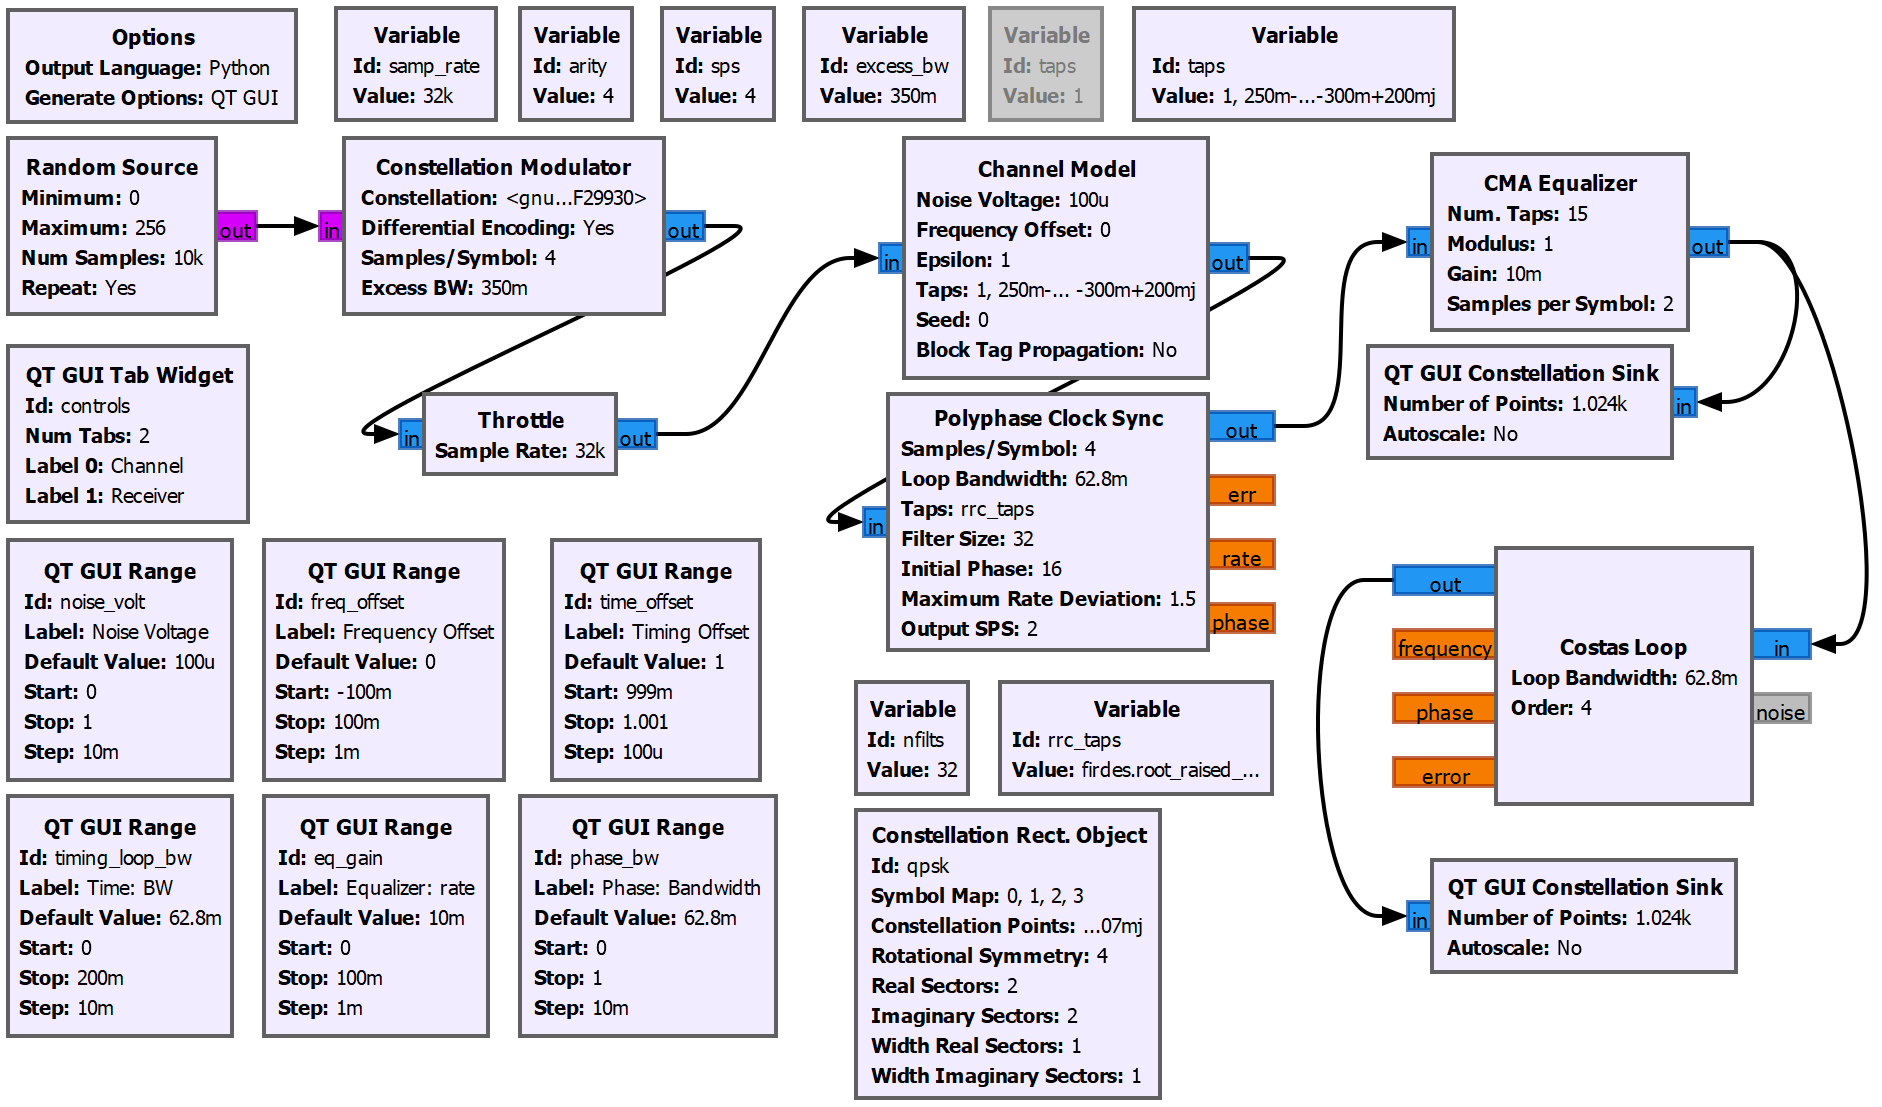
\includegraphics[width=0.75\textwidth]{6_1.png}
		\caption{mpsk\_stage5 граф}
		\label{fig:6.1}
	\end{figure}
	
	\begin{figure}[H]
		\centering
		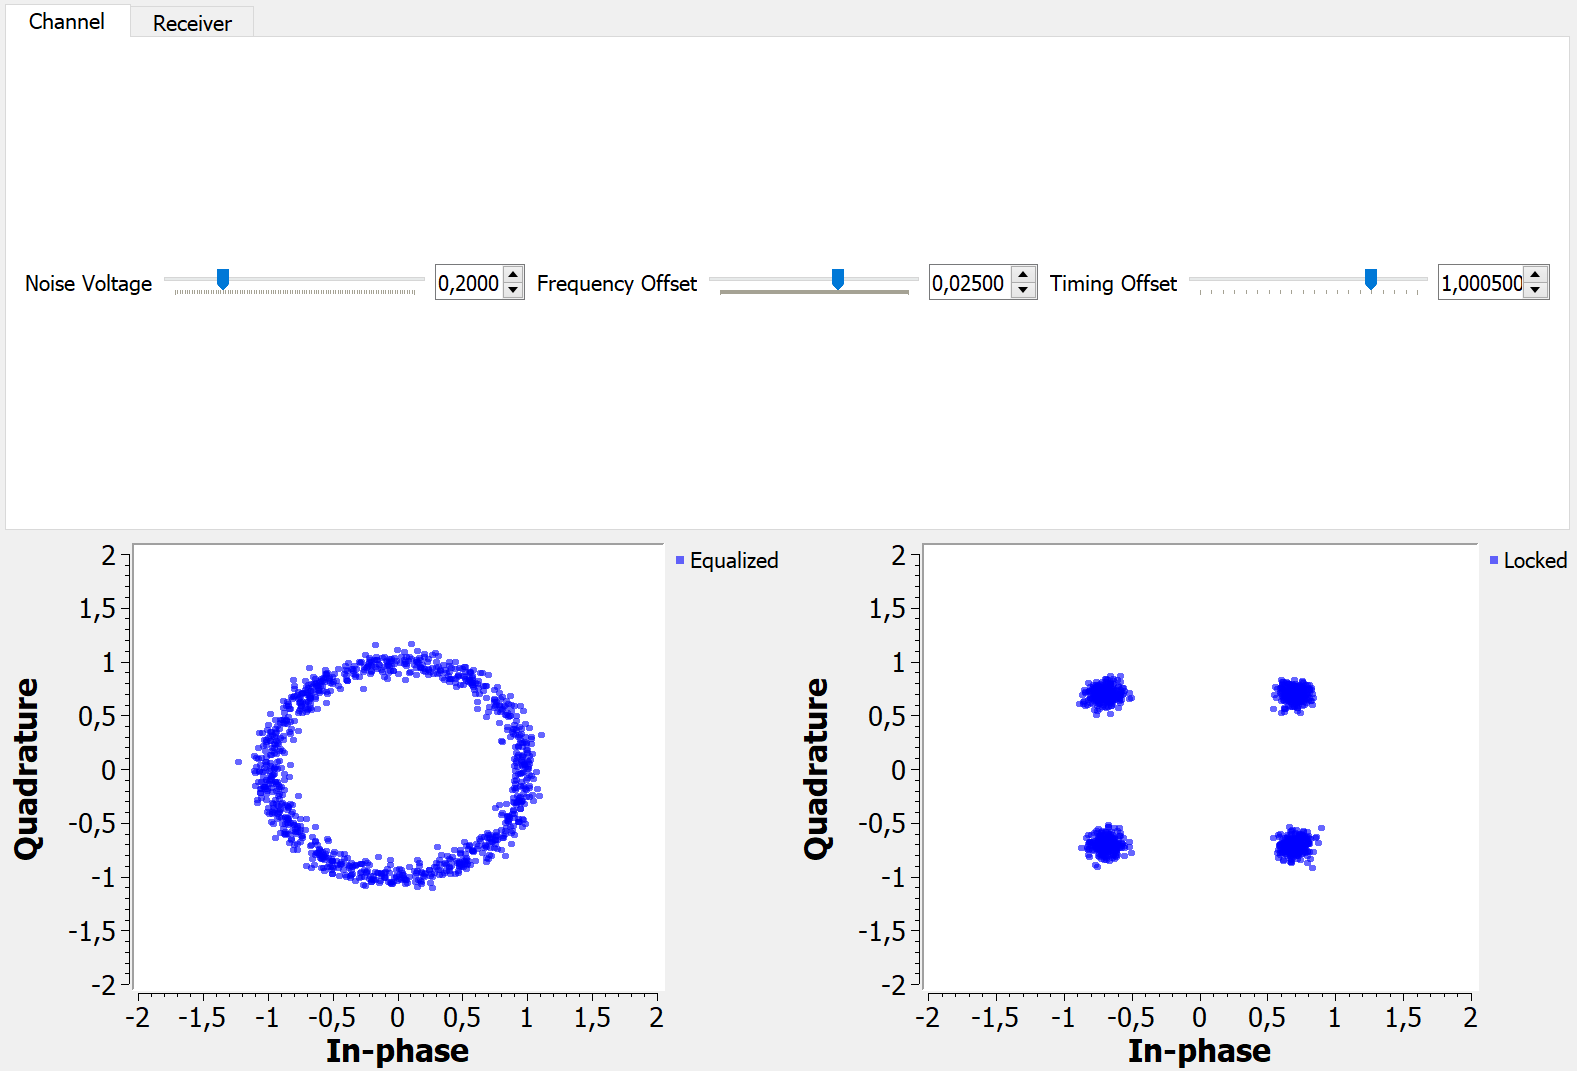
\includegraphics[width=0.75\textwidth]{6_2.png}
		\caption{Результат работы \texttt{Costas Loop}}
		\label{fig:6.2}
	\end{figure}

	
	Видим, что в результате обработки сигнал избавился от искажений, хотя небольшой шум остался.
	
	
	\section{Декодирование}
	
	Теперь попробуем декодировать сигнал. Вставим \texttt{Constellation Decoder} после \texttt{Costas Loop} и изменим параметр в \texttt{Differential} на \texttt{false} в блоке \texttt{Constellation Modulator}, тем самым выключив дифференциальное кодирование
	
	\begin{figure}[H]
		\centering
		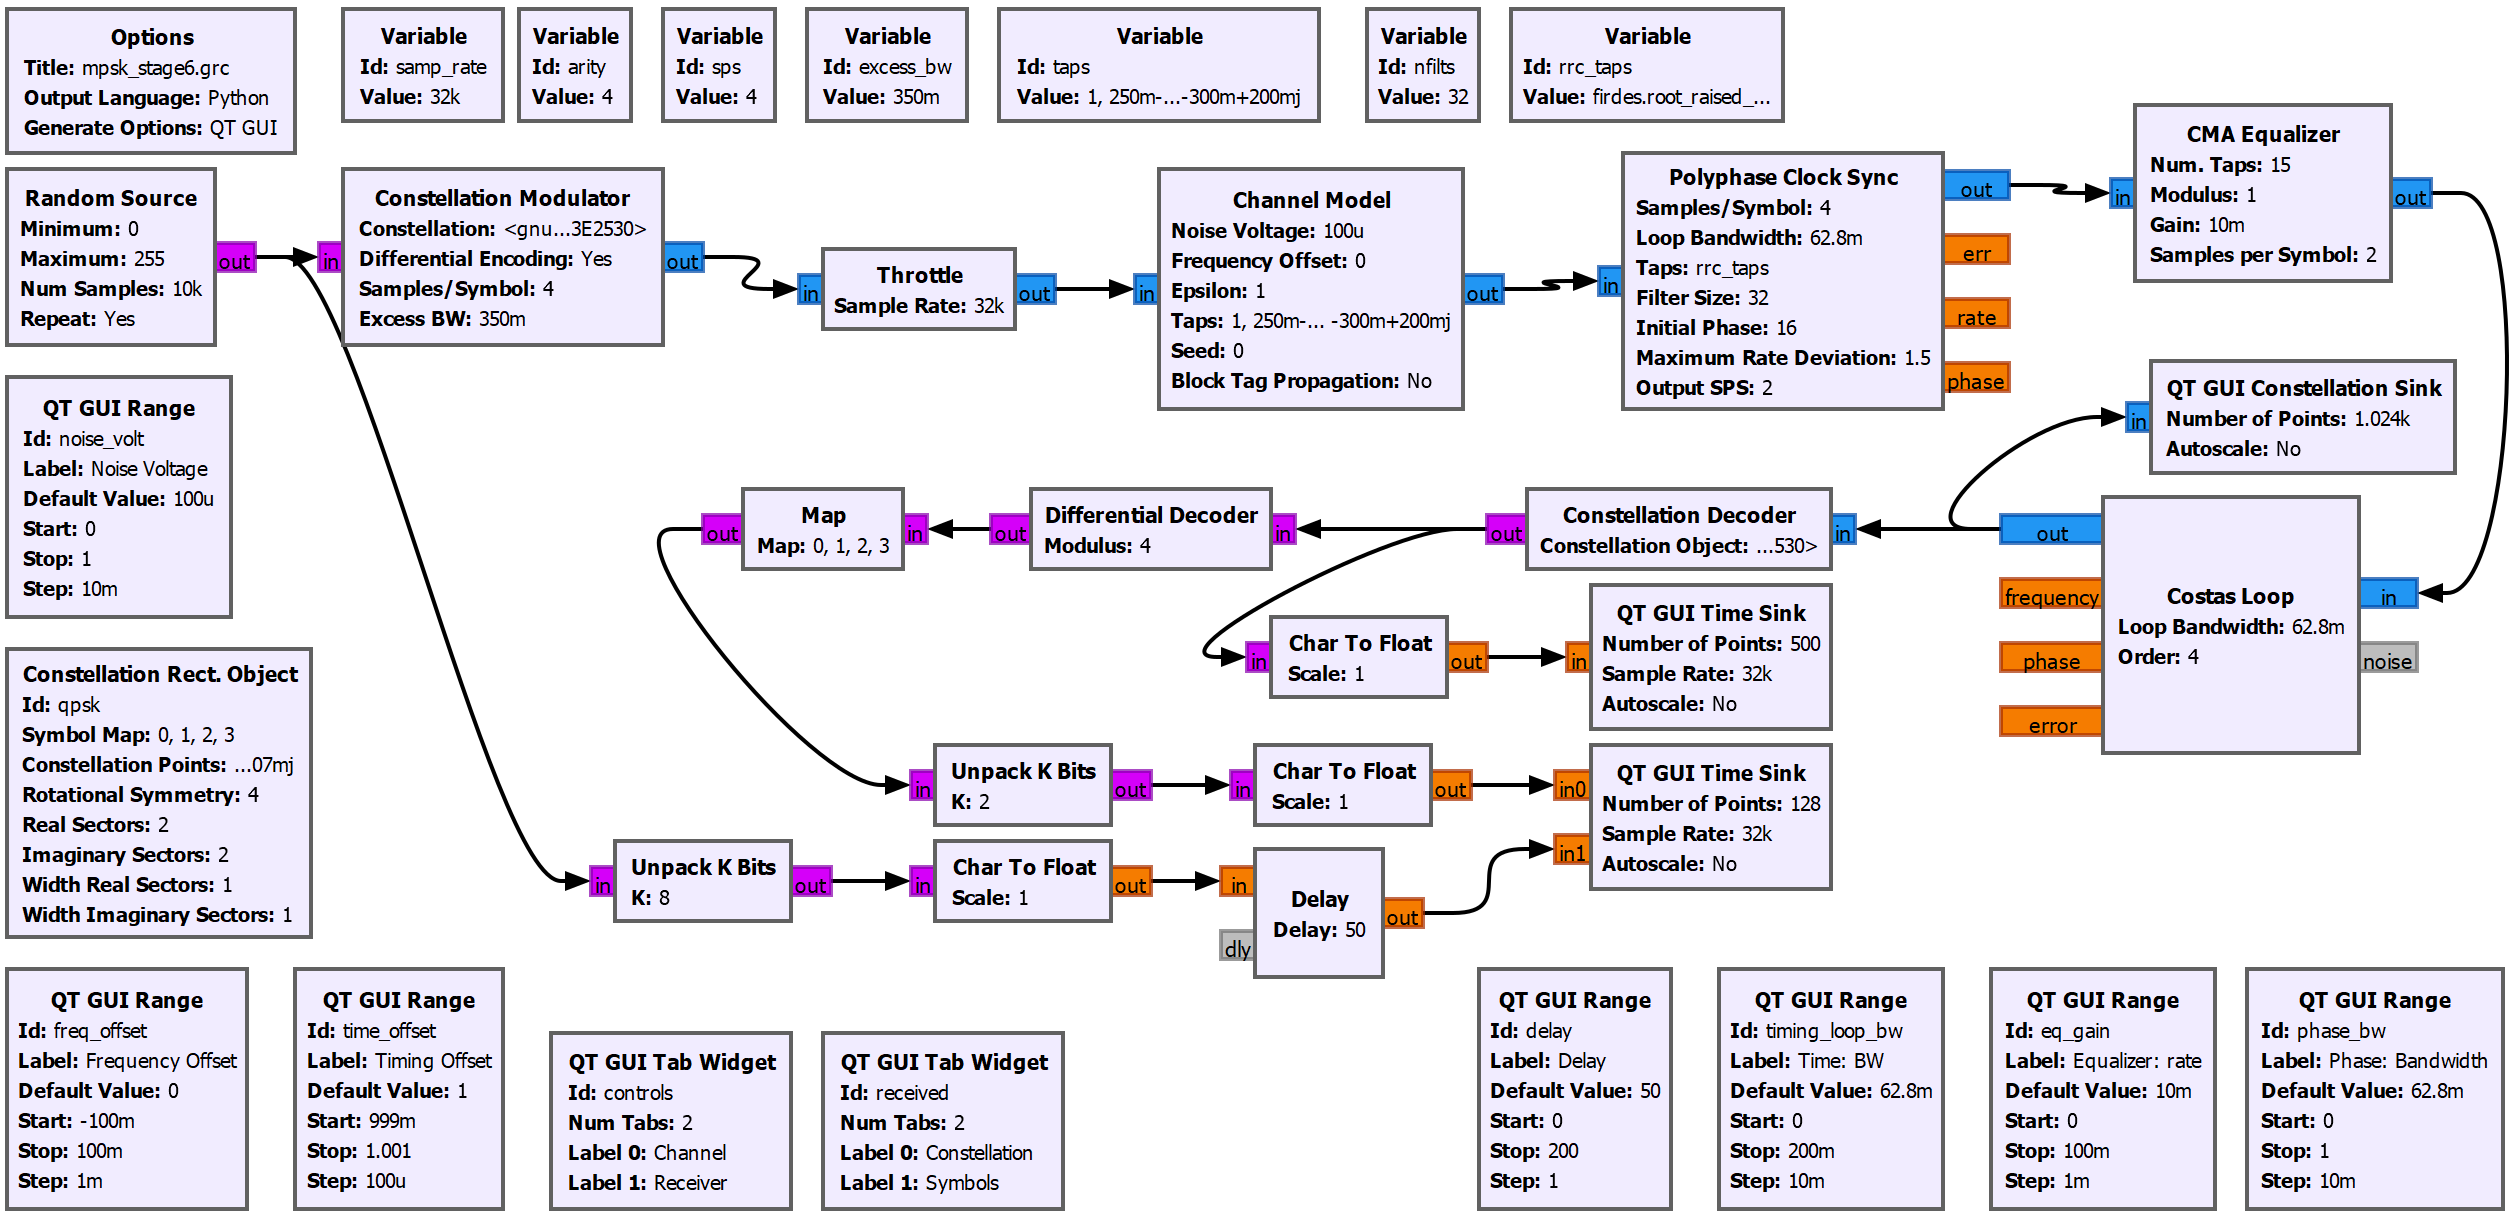
\includegraphics[width=0.75\textwidth]{7_1.png}
		\caption{mpsk\_stage6 граф}
		\label{fig:7.1}
	\end{figure}
	
	Также граф использует блок \texttt{Map} для преобразования символов из дифференциального декодера в исходные символы и блок \texttt{Unpack Bits} для распаковки полученных битов. Блок \texttt{Delay} используется для компенсации узлов, которые задерживают данные.
	
	\begin{figure}[H]
		\centering
		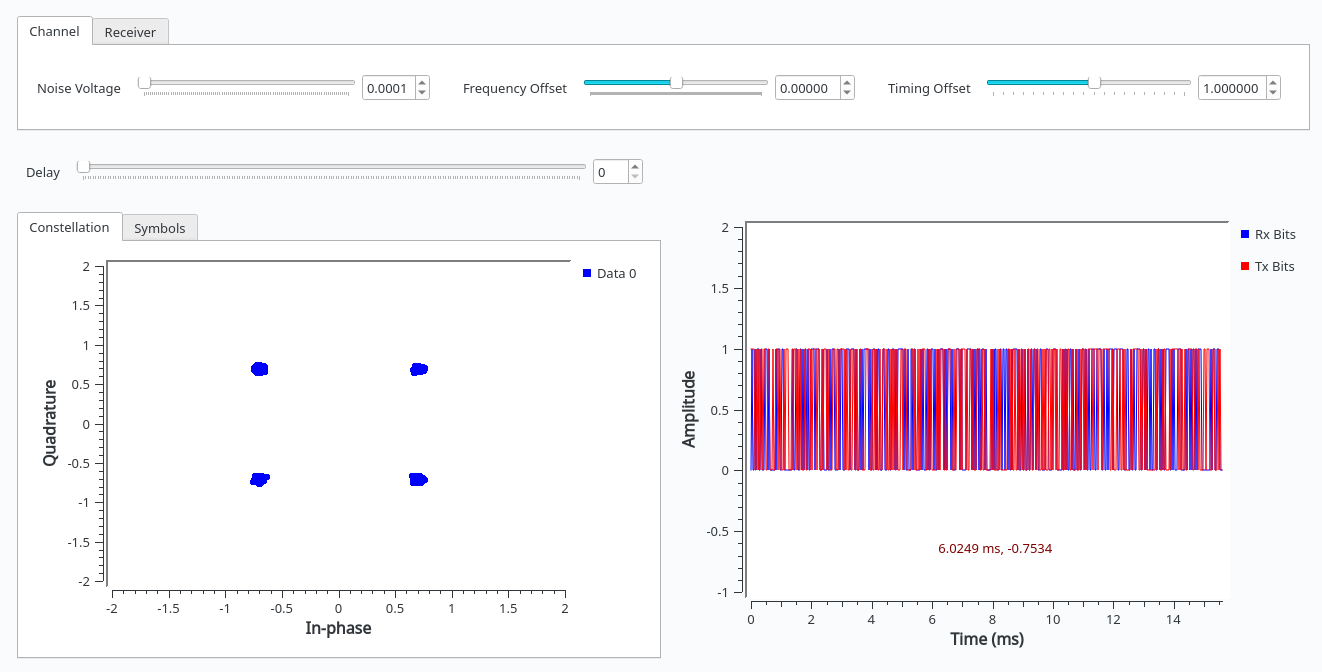
\includegraphics[width=0.75\textwidth]{7_2.png}
		\caption{Результат декодирования}
		\label{fig:7.2}
	\end{figure}
	
	Получили исходный поток данных.

	\newpage
	
	\section{Вывод}
	
	В результате выполнения работы получены навыки работы с QPSK-сигналами: мы моделировали условия передачи данных, выявляли проблемы которые могут возникнуть при передаче данных (например, канальные искажения) и рассматривали способы решения этих проблем (например, восстанавливали сигнал с помощью эквалайзеров).
	
\end{document}